\chapter{Phân tích yêu cầu và thiết kế hệ thống}
\markboth{Chương 3. Phân tích và thiết kế}{}
\section{Tác nhân và yêu cầu chức năng}
Hệ thống có hai nhóm thao tác chính. Sinh viên nhập thông tin, truy cập đề bằng mã, chuẩn bị camera, trả lời và nộp bài. Giảng viên cung cấp token quản lý để thao tác với đề thi, xem kết quả và tra cứu các sự kiện. Việc lựa chọn vai trò trên giao diện điều hướng đến màn hình phù hợp; quyền đọc dữ liệu quản lý vẫn được kiểm tra tại backend.

\begin{longtable}{@{}L{1.2cm}L{4.1cm}L{9.3cm}@{}}
\caption{Yêu cầu chức năng và phạm vi hiện có}\label{tab:req}\\
\toprule Mã & Chức năng & Phạm vi khảo sát \\\midrule\endfirsthead
\toprule Mã & Chức năng & Phạm vi khảo sát \\\midrule\endhead
FR01 & Truy cập theo vai trò & Giao diện phân luồng sinh viên/giảng viên; giảng viên sử dụng token dùng chung.\\
FR02 & Nhập đề & Nhận XLSX hoặc DOCX theo định dạng; thông báo lỗi; loại câu trùng; tạo đề nháp.\\
FR03 & Quản lý đề & Danh sách, chi tiết có đáp án cho giảng viên, công bố và xóa khi chưa có bài nộp.\\
FR04 & Lấy đề làm bài & Tìm theo mã; chỉ trả đề đã công bố trong khung giờ được cấu hình; không trả đáp án đúng.\\
FR05 & Làm và nộp bài & Lưu lựa chọn ở giao diện, đếm thời gian, gửi câu trả lời và chấm trên máy chủ.\\
FR06 & Chống nộp trùng & Một bản nộp cho mỗi cặp đề--mã sinh viên, có ràng buộc duy nhất ở CSDL.\\
FR07 & Giám sát camera & Phát hiện năm loại tín hiệu hình ảnh; chụp ảnh sự kiện và gửi backend.\\
FR08 & Sự kiện trình duyệt & Ghi nhận chuyển tab, mất tiêu điểm, thoát toàn màn hình và gửi về backend khi bài thi đang hoạt động.\\
FR09 & Tổng quan giám sát & Thống kê, tìm sinh viên, danh sách sự kiện và xem ảnh có xác thực.\\
FR10 & Kết quả & Xem điểm, số câu đúng và xuất Excel; ghép số sự kiện theo mã sinh viên, có lọc thời gian khi đề có lịch.\\
FR11 & Quản lý ảnh & Xóa ảnh riêng, xóa toàn bộ dữ liệu sự kiện qua API quản lý; tác vụ nền dọn ảnh cũ.\\
FR12 & Đa thiết bị & Web PC, Android Chrome/PWA, iOS Safari/PWA qua HTTPS; APK Android theo xác nhận tác giả.\\
FR13 & Tiếp tục thời gian & Lưu mốc bắt đầu duy nhất theo đề và mã sinh viên; gọi lại trả thời gian còn lại.\\
\bottomrule
\end{longtable}

\section{Yêu cầu phi chức năng và tiêu chí nghiệm thu}
Các yêu cầu phi chức năng dưới đây là tiêu chí cần hướng tới; không phải mọi tiêu chí đã được kiểm chứng ở phiên bản khảo sát.

\begin{longtable}{@{}L{3.2cm}L{6.2cm}L{5.2cm}@{}}
\caption{Tiêu chí chất lượng và cách kiểm tra}\\
\toprule Thuộc tính & Tiêu chí & Cách xác nhận \\\midrule\endfirsthead
\toprule Thuộc tính & Tiêu chí & Cách xác nhận \\\midrule\endhead
Tính đúng đắn & Điểm theo đáp án máy chủ; không phát đáp án đúng trong API làm bài. & Kiểm thử API và đối chiếu kết quả với dữ liệu mẫu.\\
Khả dụng giao diện & Câu hỏi dài, camera, cảnh báo và nút nộp dễ quan sát; lỗi có thông báo. & Kiểm thử màn hình thật ở nhiều độ phân giải.\\
Hiệu năng & Suy luận và thao tác không gây giật đáng kể trên thiết bị mục tiêu. & Đo thời gian suy luận, độ trễ, CPU và khung hình trên thiết bị thật.\\
Toàn vẹn dữ liệu & Không tạo hai bài nộp cho cùng đề và mã sinh viên; thời gian nhất quán. & Kiểm thử nộp trùng, tranh chấp đồng thời và chuyển đổi múi giờ.\\
Bảo mật & Chỉ giảng viên có quyền xem dữ liệu quản lý và ảnh. & Kiểm tra các tuyến với token thiếu, sai và hợp lệ; đánh giá phiên đăng nhập.\\
Riêng tư & Thu thập tối thiểu; ảnh có thời hạn lưu và có thể xóa. & Rà soát luồng dữ liệu, tác vụ dọn ảnh và quy trình thông báo cho sinh viên.\\
Khả năng tái lập & Chốt phiên bản mã, phụ thuộc, mô hình và dữ liệu kiểm thử. & Dựng lại môi trường từ commit và ghi nhận phiên bản thực dùng.\\
\bottomrule
\end{longtable}

\section{Các ca sử dụng chính}
\subsection{UC01: Giảng viên tạo và công bố đề}
Tiền điều kiện là giảng viên có token hợp lệ và tệp đề theo mẫu. Giảng viên chọn tệp, nhập tên đề và tùy chọn mã đề. Backend kiểm tra kích thước, định dạng và nội dung; các câu hợp lệ được lưu dưới một đề ở trạng thái nháp. Giảng viên xem thông tin và lỗi nhập, sau đó cấu hình thời lượng, ngưỡng đạt và xáo trộn trước khi công bố.

Nếu tệp không có câu hợp lệ hoặc vượt giới hạn số câu, hệ thống không được coi là đã tạo thành công một đề dùng được. Nếu có câu không hợp lệ nhưng vẫn còn câu hợp lệ, người dùng cần đọc thông báo nhập để tránh tưởng rằng toàn bộ tệp đã được chấp nhận. Sau khi công bố, mã đề trở thành đầu vào cho luồng sinh viên.

\subsection{UC02: Sinh viên làm và nộp bài}
Sinh viên khai báo thông tin, nhập mã đề, xem phần chuẩn bị và bắt đầu làm bài. Giao diện tải câu hỏi không kèm đáp án đúng, xin quyền camera và khởi tạo mô hình. Các lựa chọn trả lời được giữ trong trạng thái của trang. Khi nộp, máy chủ đọc câu hỏi gốc, so sánh đáp án và lưu kết quả trong giao dịch.

Luồng ngoại lệ gồm mã đề sai, đề chưa công bố, ngoài lịch mở đề, camera bị từ chối, mô hình không tải được, mạng gián đoạn hoặc mã sinh viên đã nộp bài. Với mã đã nộp, backend trả xung đột thay vì tạo bản nộp thứ hai. Máy chủ đã lưu mốc bắt đầu trong exam\_starts. Gọi lại API bắt đầu khôi phục thời gian còn lại khi dịch vụ phản hồi, nhưng không khôi phục các đáp án vốn chỉ lưu trong trạng thái React; API nộp chưa cưỡng chế deadline.

\subsection{UC03: Giảng viên xem xét sự kiện}
Giảng viên mở tổng quan, lọc hoặc tìm sinh viên rồi xem danh sách các nhãn nghi vấn. Với sự kiện còn ảnh, giao diện lấy ảnh qua yêu cầu có token và hiển thị để giảng viên đối chiếu. Nếu ảnh đã được dọn, bản ghi thời gian và loại sự kiện vẫn tồn tại.

Hậu điều kiện của ca sử dụng hiện tại là người dùng đã tra cứu được thông tin. Dự án chưa có quy trình xét duyệt ``xác nhận vi phạm'', ``bác bỏ cảnh báo'' hoặc khiếu nại được lưu thành một hồ sơ riêng. Vì vậy, không nên đồng nhất việc xuất hiện một hàng trong danh sách với quyết định kỷ luật đã được xác lập.

\section{Kiến trúc tổng thể}


Hai vai trò cùng sử dụng ứng dụng frontend, nhưng truy cập các thành phần khác nhau. Backend là điểm tập trung dữ liệu. Mô hình AI thực thi ở trình duyệt sinh viên; khi phát sinh sự kiện, ảnh thu nhỏ và metadata được gửi tới API. Tác vụ APScheduler chạy phía backend để dọn ảnh theo thời hạn.

Trong môi trường phát triển, Vite chuyển tiếp đường dẫn \src{/api} sang cổng 8000. Trong bản triển khai tunnel, FastAPI trực tiếp phục vụ frontend/dist và SPA fallback; web và API cùng origin, không cần Vite để phục vụ bản build. Camera trên web cũng cần môi trường nguồn tin cậy như localhost khi phát triển hoặc HTTPS khi triển khai.

\section{Thiết kế mô-đun}
\begin{longtable}{@{}L{4.8cm}L{10.2cm}@{}}
\caption{Phân chia mô-đun trong mã nguồn}\\
\toprule Mô-đun & Trách nhiệm \\\midrule\endfirsthead
\toprule Mô-đun & Trách nhiệm \\\midrule\endhead
\src{App.jsx} & Điều hướng vai trò, thông tin truy cập và trạng thái cấp ứng dụng.\\
\src{StudentGateway.jsx} & Nhập mã đề, chuẩn bị thông tin trước khi vào phòng thi.\\
\src{StudentExam.jsx} & Giao diện câu hỏi, timer, camera, mô hình, quy tắc cảnh báo và nộp bài.\\
\src{useBrowserLockdown.js} & Listener sự kiện trang, giới hạn thao tác và callback gửi sự kiện khi đang thi.\\
\src{ProctorDashboard.jsx} & Tổng quan, dữ liệu sinh viên, sự kiện và ảnh có token.\\
\src{ExamManagement.jsx} & Nhập, công bố, xem kết quả và xuất dữ liệu đề thi.\\
\src{ModalShell.jsx} & Khung hộp thoại dùng lại cho các thao tác giao diện.\\
\src{main.py} & API sự kiện, thống kê, ảnh, health và khởi tạo ứng dụng.\\
\src{exams_router.py} & API vòng đời đề, lấy đề, chấm và xuất kết quả.\\
\src{exam_parser.py} & Phân tích XLSX/DOCX, kiểm tra câu hỏi và loại trùng.\\
\src{database.py} & Engine, session, các bảng và tuần tự hóa dữ liệu.\\
\src{auth.py} & Đọc token và xác minh quyền giám thị.\\
\src{scheduler.py} & Tác vụ xóa ảnh hết hạn, giữ metadata.\\
\bottomrule
\end{longtable}

\section{Thiết kế cơ sở dữ liệu}
\subsection{Mô hình quan hệ}


Bảng \src{exams} sở hữu tập câu hỏi, các mốc bắt đầu và các bài nộp. Bảng \src{exam_starts} lưu duy nhất giờ bắt đầu cho mỗi cặp đề--mã sinh viên; bảng này không phải phiên đăng nhập hay nơi lưu nháp đáp án. Bảng \src{submission_answers} lưu từng lựa chọn gắn với câu hỏi gốc và một bản nộp. Ràng buộc duy nhất trên cặp \src{exam_id, student_id} trong bảng bài nộp hạn chế ghi hai lần. Bảng \src{violations} hiện đứng riêng, không có \src{exam_id} hoặc khóa ngoại đến một phiên làm bài.

Thiết kế này đơn giản hóa ghi sự kiện, nhưng khi cùng một mã sinh viên tham gia nhiều đề, việc quy một sự kiện về đúng bài thi phụ thuộc điều kiện thời gian. Nếu đề không có thời điểm mở và đóng, phép tổng hợp có thể tính cả sự kiện của lần thi khác. Hướng cải tiến là cấp mã phiên thi tại backend và bắt buộc mọi sự kiện tham chiếu phiên đó.

\subsection{Các trường và ràng buộc quan trọng}
\begin{longtable}{@{}L{3cm}L{7.5cm}L{4.1cm}@{}}
\caption{Tóm tắt từ điển dữ liệu}\\
\toprule Bảng & Nhóm trường chính & Ràng buộc / ý nghĩa \\\midrule\endfirsthead
\toprule Bảng & Nhóm trường chính & Ràng buộc / ý nghĩa \\\midrule\endhead
exams & id; exam\_code; title; duration\_minutes; pass\_score; shuffle\_questions; status; start\_time; end\_time; created\_by; created\_at. & Mã đề duy nhất; trạng thái mặc định DRAFT; lịch thi có thể rỗng.\\
exam\_starts & id; exam\_id; student\_id; started\_at. & FK tới exams; UNIQUE(exam\_id, student\_id).\\
questions & id; exam\_id; order\_index; content; option\_a/b/c/d; correct\_option; score\_weight. & Thuộc một đề; lưu đáp án chuẩn tại máy chủ.\\
\src{exam_submissions} & id; exam\_id; student\_id; student\_name; started\_at; submitted\_at; total\_score; correct\_count; total\_questions; status. & UNIQUE theo đề và mã sinh viên. started\_at được lấy từ exam\_starts nếu có bản ghi bắt đầu.\\
\src{submission_answers} & id; submission\_id; question\_id; selected\_option; is\_correct. & Liên kết bản nộp và câu hỏi; lựa chọn có thể rỗng.\\
violations & id; student\_id; student\_name; violation\_type; captured\_at; image\_path; created\_at. & Chỉ mục theo mã sinh viên, loại và thời điểm; ảnh có thể rỗng hoặc đã bị dọn.\\
\bottomrule
\end{longtable}

Tên bảng và trường phản ánh cài đặt hiện có. Các cột chuỗi có khai báo độ dài trong mô hình ORM, nhưng không nên chỉ dựa vào khai báo này để bảo đảm kiểm tra đầu vào trên SQLite. Các điều kiện dữ liệu quan trọng cần được kiểm tra ở mô hình yêu cầu, nghiệp vụ hoặc ràng buộc CSDL phù hợp.

\section{Luồng dữ liệu và trạng thái}
\subsection{Luồng nộp bài}


Câu trả lời được tham chiếu bằng ID câu hỏi thay vì vị trí trên giao diện, nên có thể xáo trộn thứ tự câu mà vẫn chấm theo đúng câu gốc. Tuy nhiên, nếu một payload lặp ID câu hỏi, cách tạo ánh xạ ở backend làm lựa chọn xuất hiện sau ghi đè lựa chọn trước. Đây là hành vi hiện tại cần được biết khi xây dựng kiểm thử biên; hướng chặt chẽ hơn là từ chối yêu cầu trùng ID.

\subsection{Vòng đời đề thi và dữ liệu giám sát}
Đề mới tạo có trạng thái DRAFT; thao tác công bố chuyển thành PUBLISHED. Mã nguồn định nghĩa CLOSED và có nhánh kiểm tra trạng thái này, nhưng chưa có tuyến riêng để đóng đề. Cần phân biệt sự tồn tại của một hằng trạng thái với một quy trình chuyển trạng thái đầy đủ trên giao diện và API.

Sự kiện giám sát đi từ khung hình đến nhãn, được kiểm tra khoảng nghỉ, thêm vào nhật ký cục bộ và gửi mạng. Ảnh được tách ra tệp, còn thông tin tra cứu ở CSDL. Khi dọn ảnh, metadata vẫn còn. Do đó, số ``tổng vi phạm'' và số ``có ảnh chứng cứ'' có thể khác nhau mà không nhất thiết là lỗi thống kê.

\section{Thiết kế an toàn và các ranh giới tin cậy}
Các API quản lý và đọc ảnh kiểm tra token giám thị; API sinh viên lấy đề, nộp bài và gửi sự kiện không yêu cầu token này. Cách tách quyền giúp sinh viên không cần biết bí mật quản lý, nhưng chưa cung cấp chứng thực riêng cho sinh viên. Một phía gửi có thể tự chọn mã sinh viên nếu không có lớp bảo vệ bổ sung.

Token là bí mật dùng chung, không phải JWT và không có vai trò chi tiết theo từng giảng viên. Backend chấp nhận token qua header hoặc query; sử dụng header phù hợp hơn để hạn chế xuất hiện bí mật trong URL. Giao diện lấy ảnh bằng fetch có token rồi tạo URL đối tượng, thay vì công khai thư mục ảnh. Cơ chế này kiểm soát truy cập ảnh, nhưng không thay thế chính sách cấp quyền, quản lý phiên và nhật ký truy cập khi đưa vào vận hành thật.

\section{Bộ sơ đồ hệ thống cập nhật}
Các sơ đồ dưới đây biểu diễn commit khảo sát ngày 01/10/2026. Màu xanh dương thể hiện máy khách, xanh lá là xử lý máy chủ, vàng là dữ liệu, tím là hạ tầng ngoài và cam là điều kiện hoặc ngoại lệ. Sơ đồ ngữ cảnh, DFD và ERD bổ trợ cho UML; không gọi tất cả các sơ đồ là UML. Tệp draw.io kèm theo cho phép sửa nhãn, nút và đường nối.

\clearpage
\subsection{Ngữ cảnh hệ thống}
Ngữ cảnh xác định hai tác nhân và nguồn tài nguyên AI bên ngoài. Cloudflare được thể hiện ở sơ đồ triển khai vì là hạ tầng truyền dẫn, không phải tác nhân nghiệp vụ.
\begin{figure}[H]
\centering
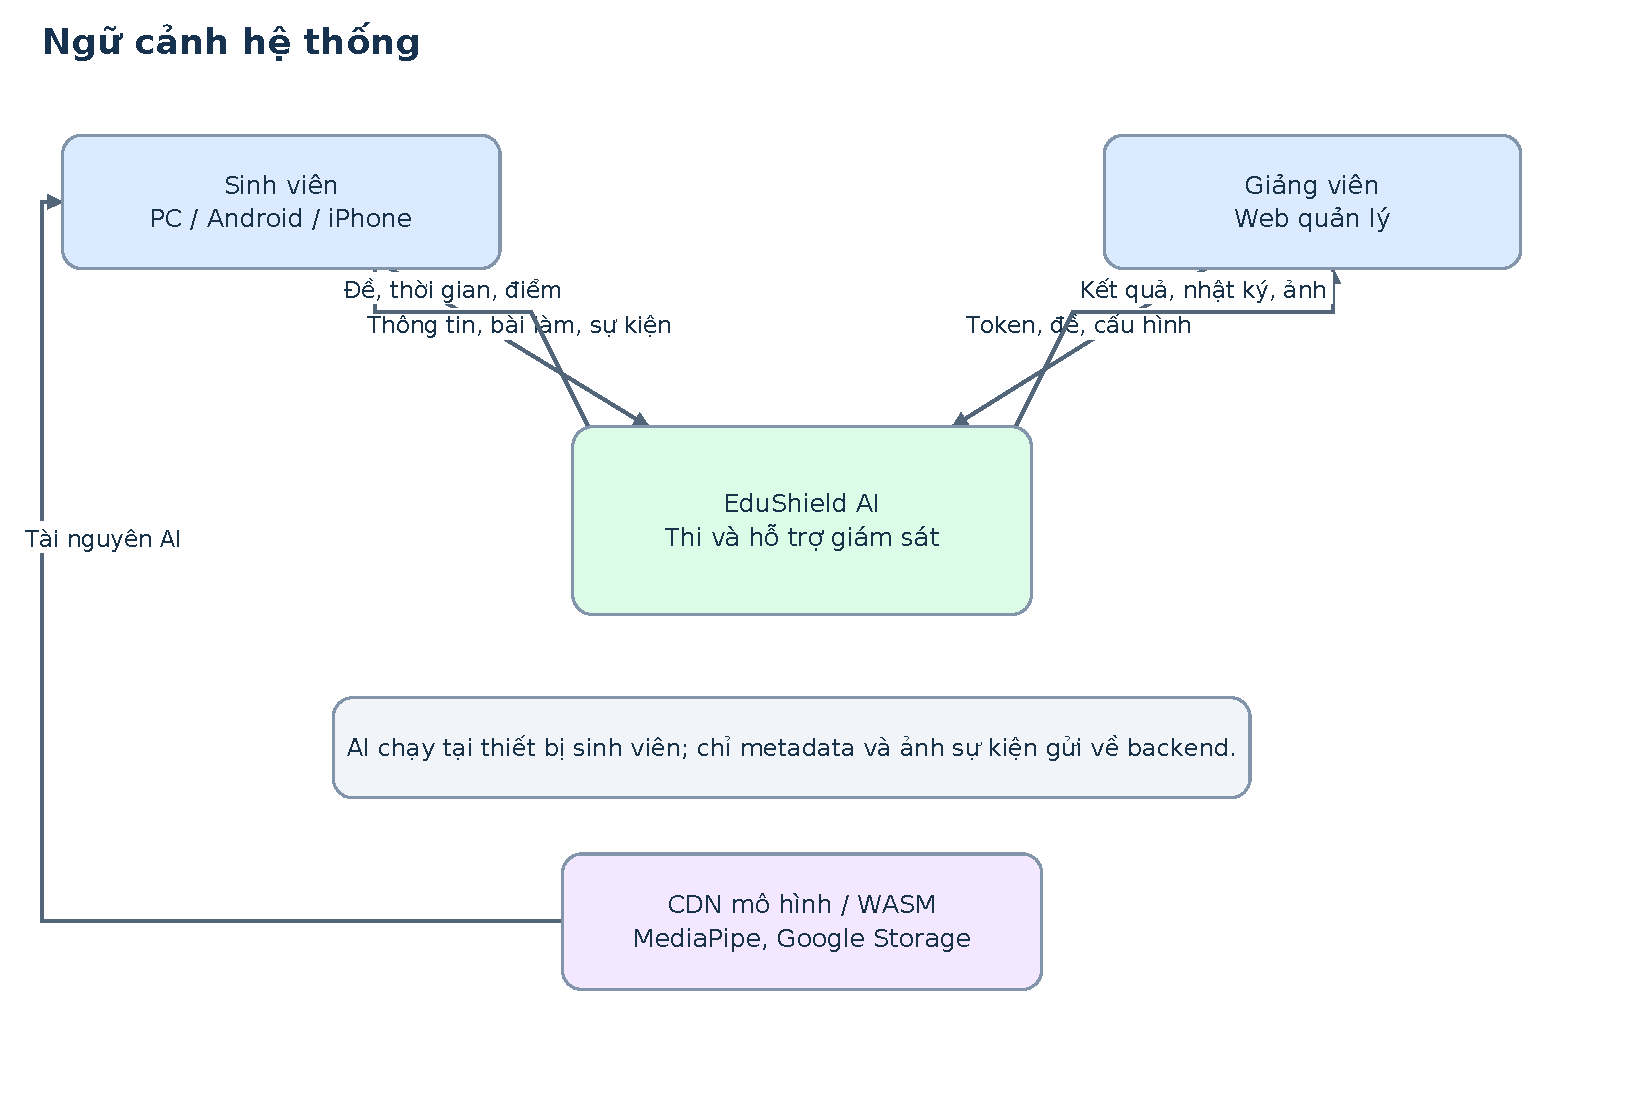
\includegraphics[width=\textwidth,height=0.70\textheight,keepaspectratio]{diagrams/01-context.pdf}
\caption{Ngữ cảnh hệ thống của EduShield AI.}\label{fig:01-context}
\end{figure}

\clearpage
\subsection{Ca sử dụng chính}
Ca sử dụng bao quát thao tác của sinh viên và giảng viên. Chọn vai trò ở giao diện không cấp quyền quản lý; backend vẫn xác minh token.
\begin{figure}[H]
\centering
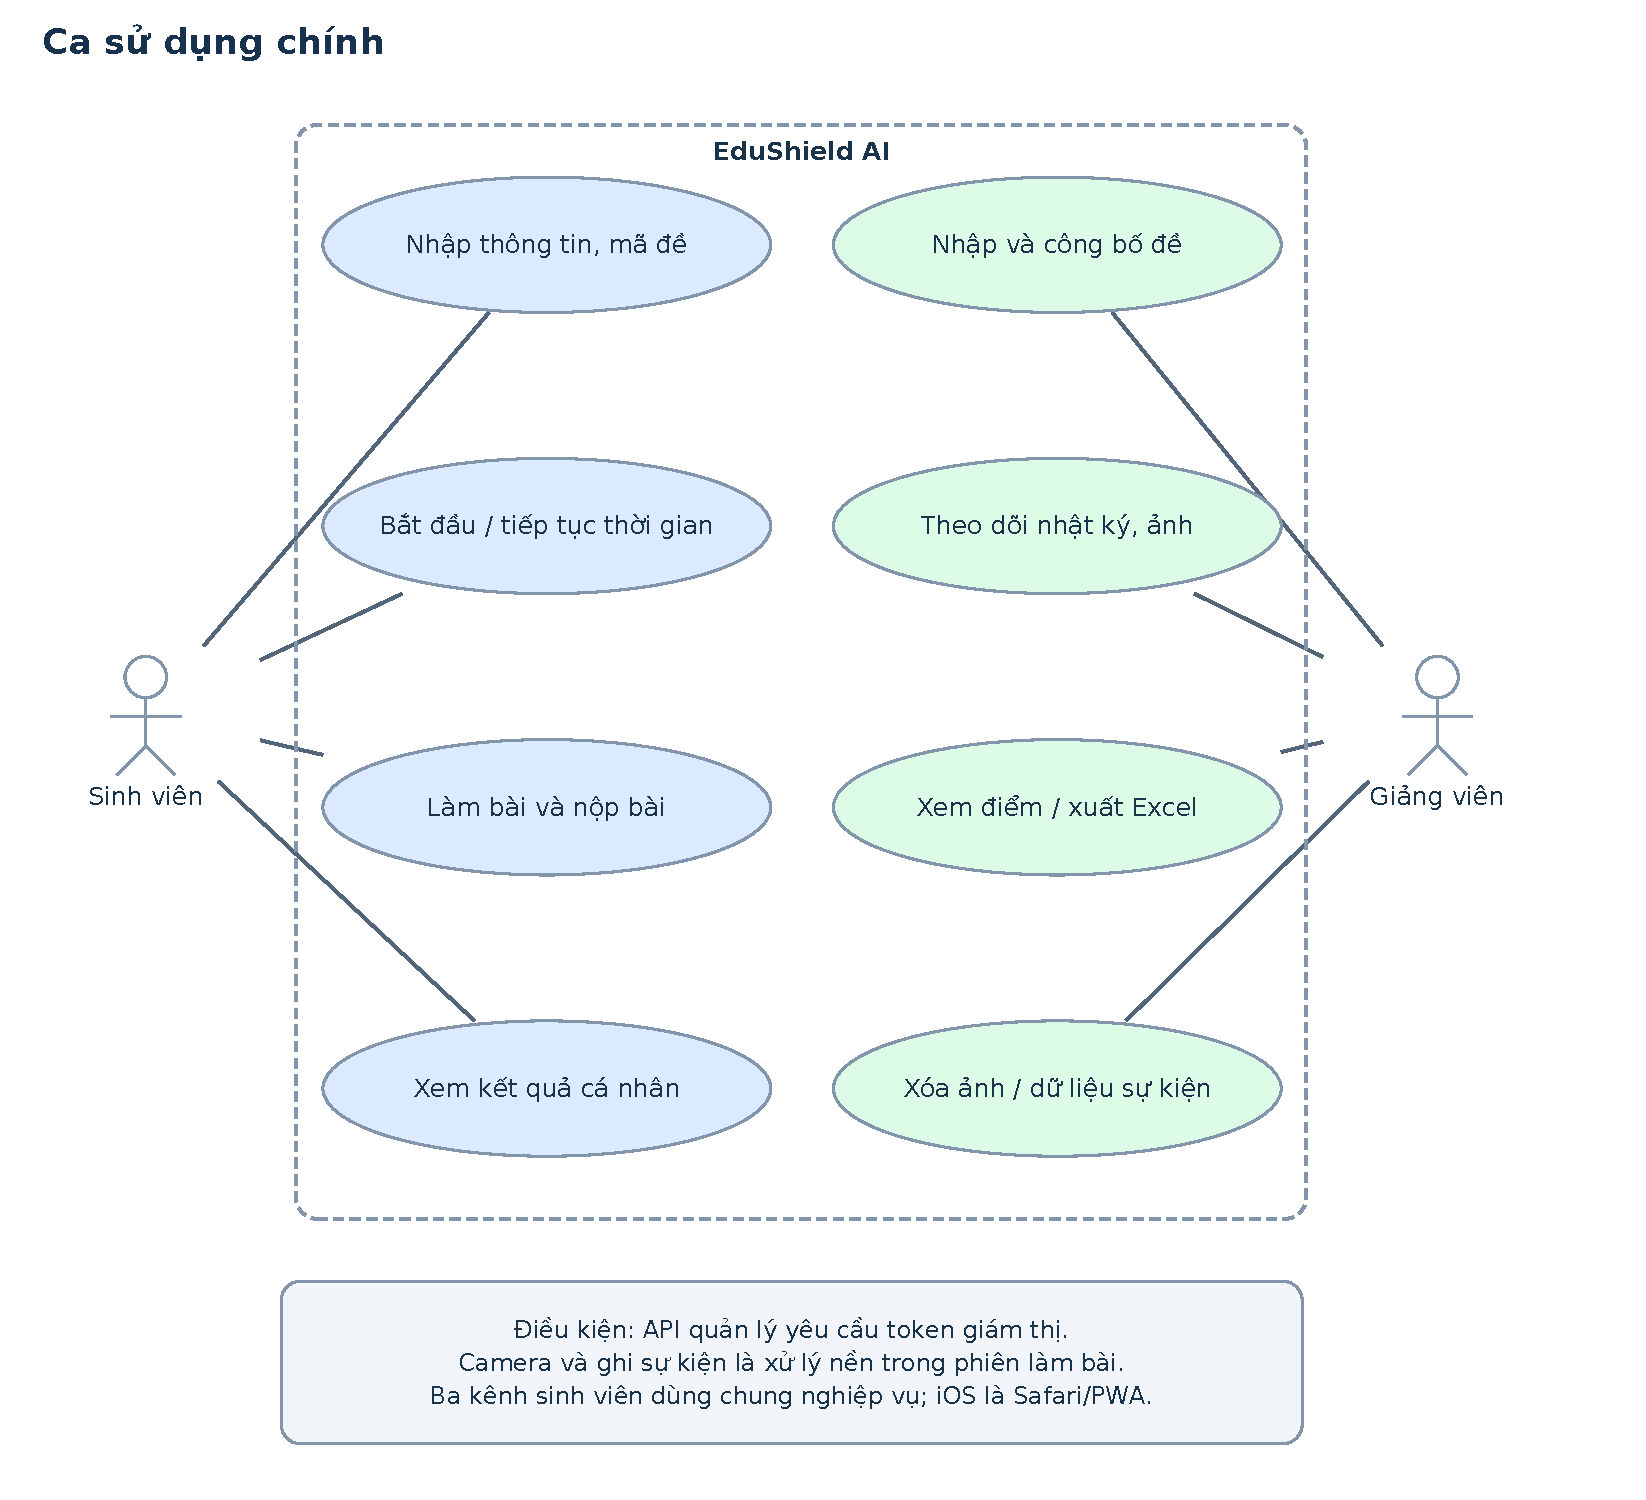
\includegraphics[width=\textwidth,height=0.70\textheight,keepaspectratio]{diagrams/02-usecase.pdf}
\caption{Ca sử dụng chính của EduShield AI.}\label{fig:02-usecase}
\end{figure}

\clearpage
\subsection{Cấu trúc thành phần}
Sơ đồ thành phần thể hiện trách nhiệm chính và phụ thuộc mức mô-đun, không phải sơ đồ mọi lời gọi hàm. Các máy khách chia sẻ API nghiệp vụ.
\begin{figure}[H]
\centering
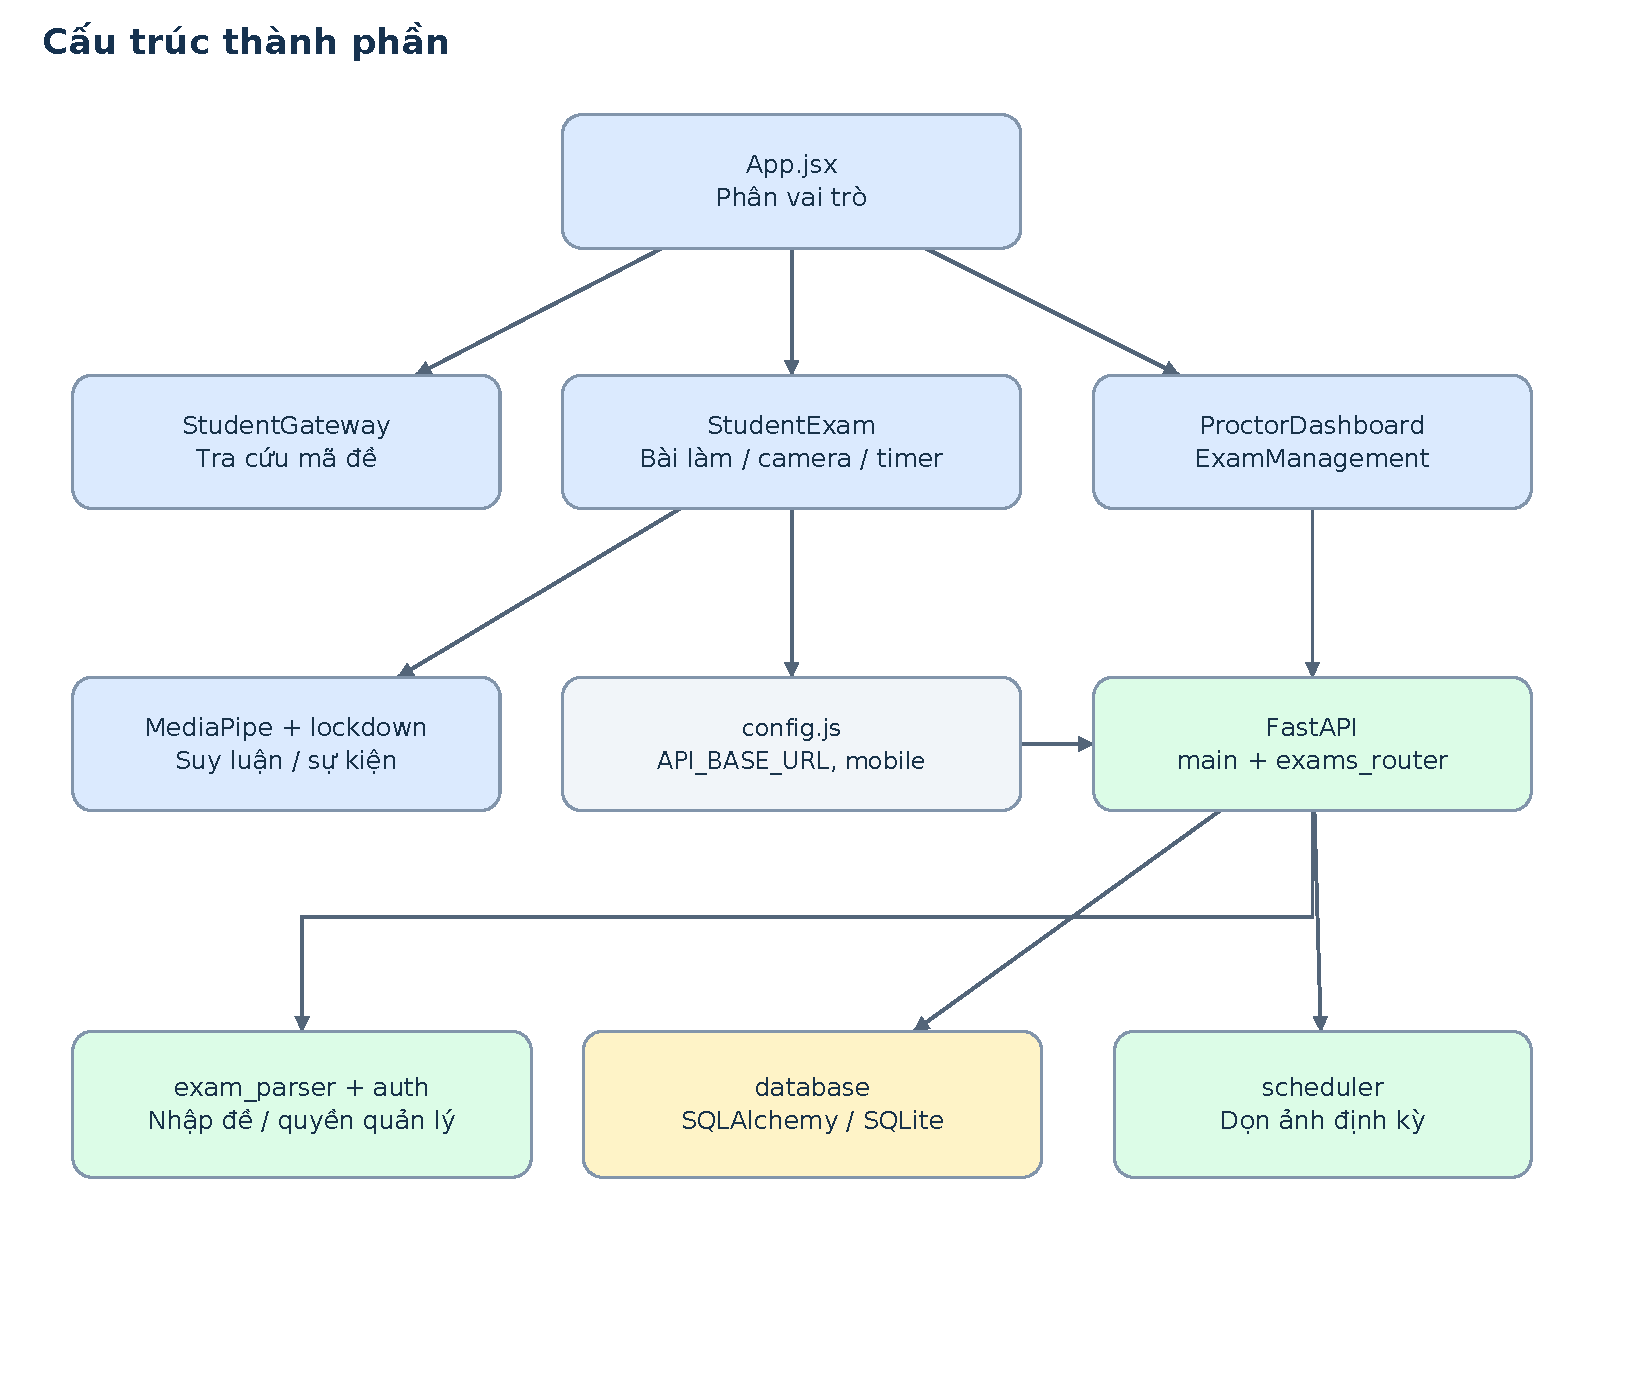
\includegraphics[width=\textwidth,height=0.70\textheight,keepaspectratio]{diagrams/03-components.pdf}
\caption{Cấu trúc thành phần của EduShield AI.}\label{fig:03-components}
\end{figure}

\clearpage
\subsection{Triển khai HTTPS đa thiết bị}
Web và API được phục vụ cùng origin trên FastAPI. APK là kênh đã chạy theo xác nhận tác giả nhưng chưa có nguồn native để tái lập trong repo main. iOS là Safari/PWA.
\begin{figure}[H]
\centering
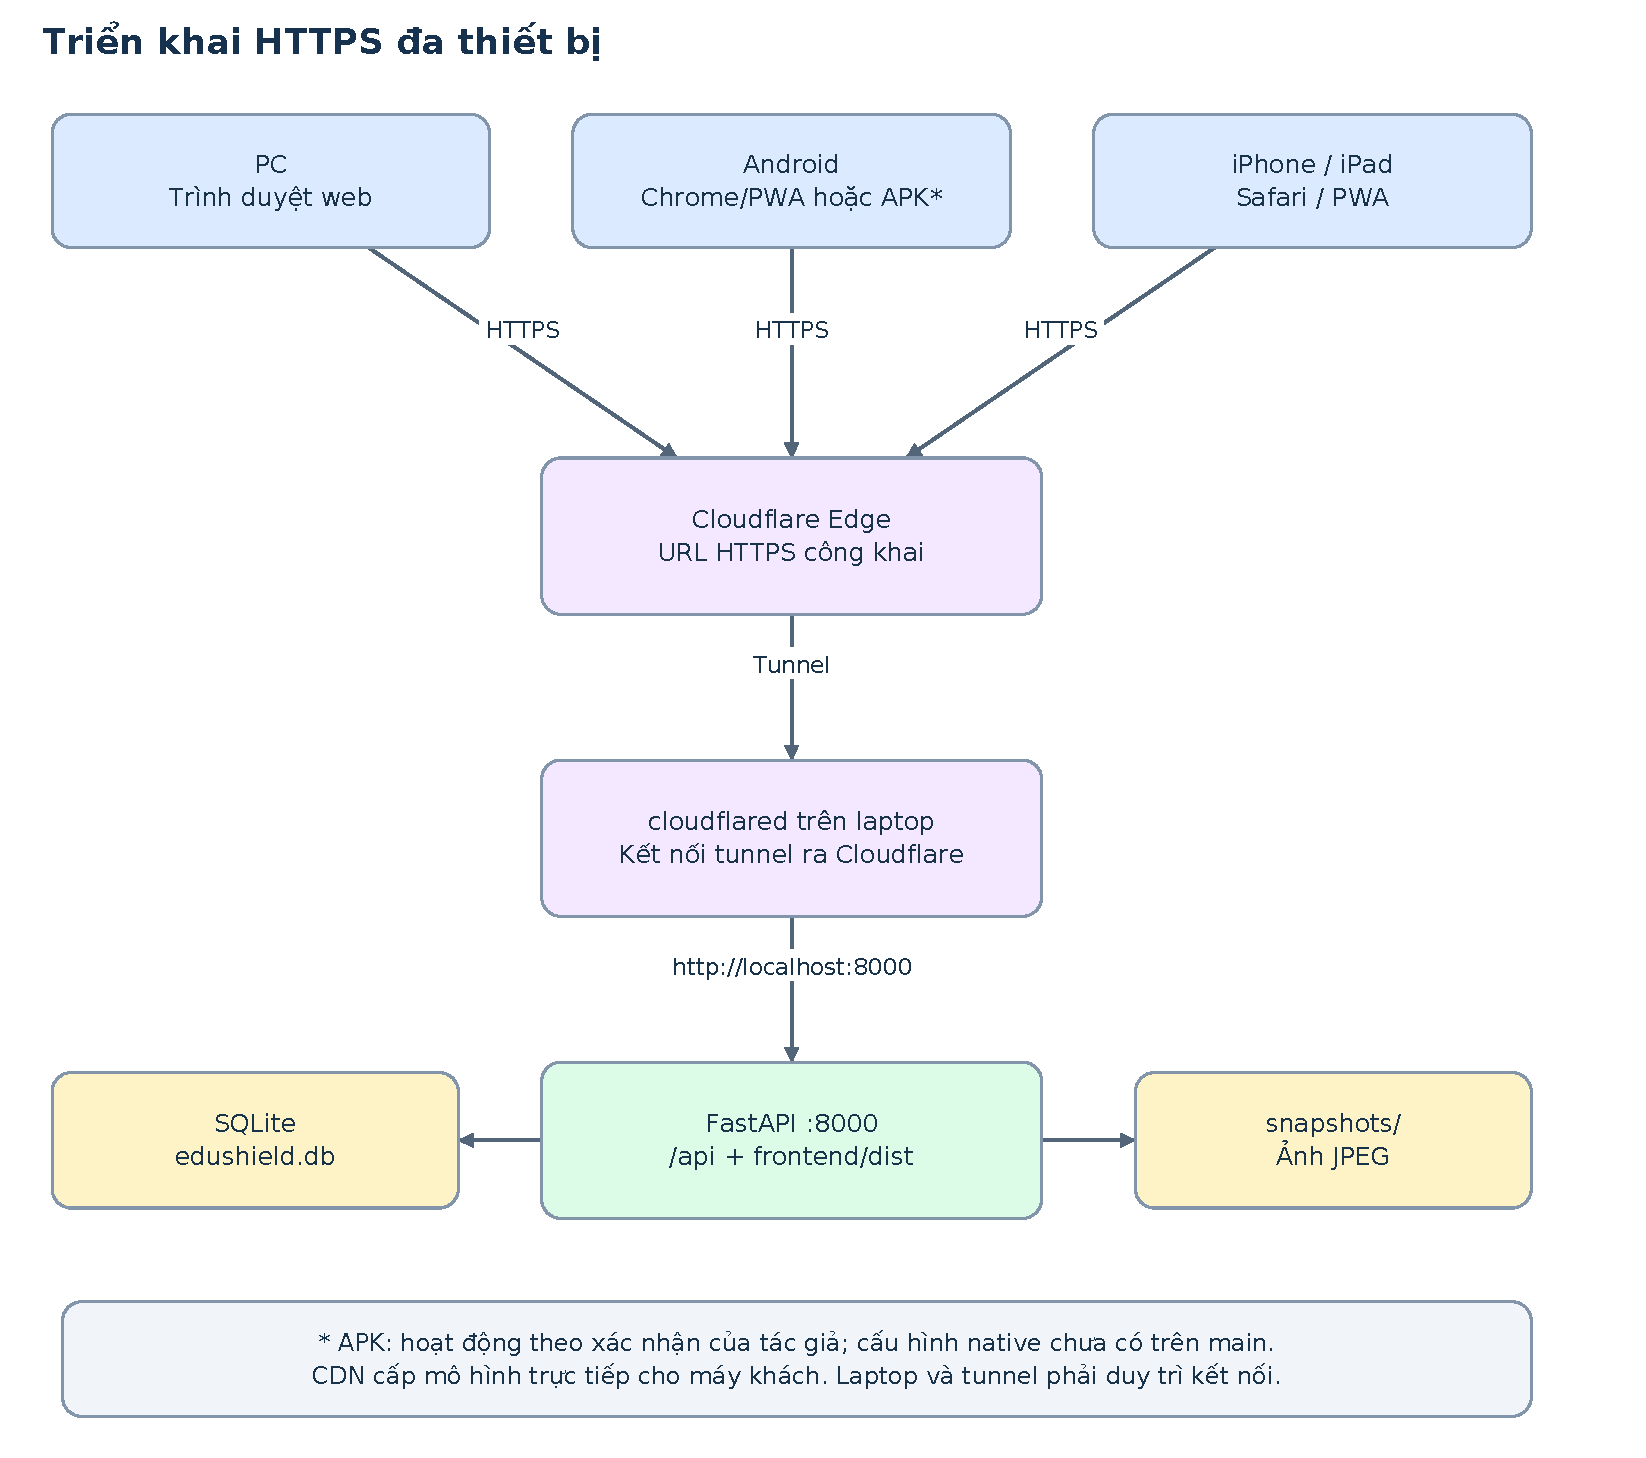
\includegraphics[width=\textwidth,height=0.70\textheight,keepaspectratio]{diagrams/04-deployment.pdf}
\caption{Triển khai HTTPS đa thiết bị của EduShield AI.}\label{fig:04-deployment}
\end{figure}

\clearpage
\subsection{Luồng dữ liệu mức 1}
DFD mức 1 phân rã các xử lý nghiệp vụ và kho dữ liệu. Suy luận hình ảnh nằm ở máy khách; backend nhận sự kiện đã xử lý thay vì nhận luồng video liên tục.
\begin{figure}[H]
\centering
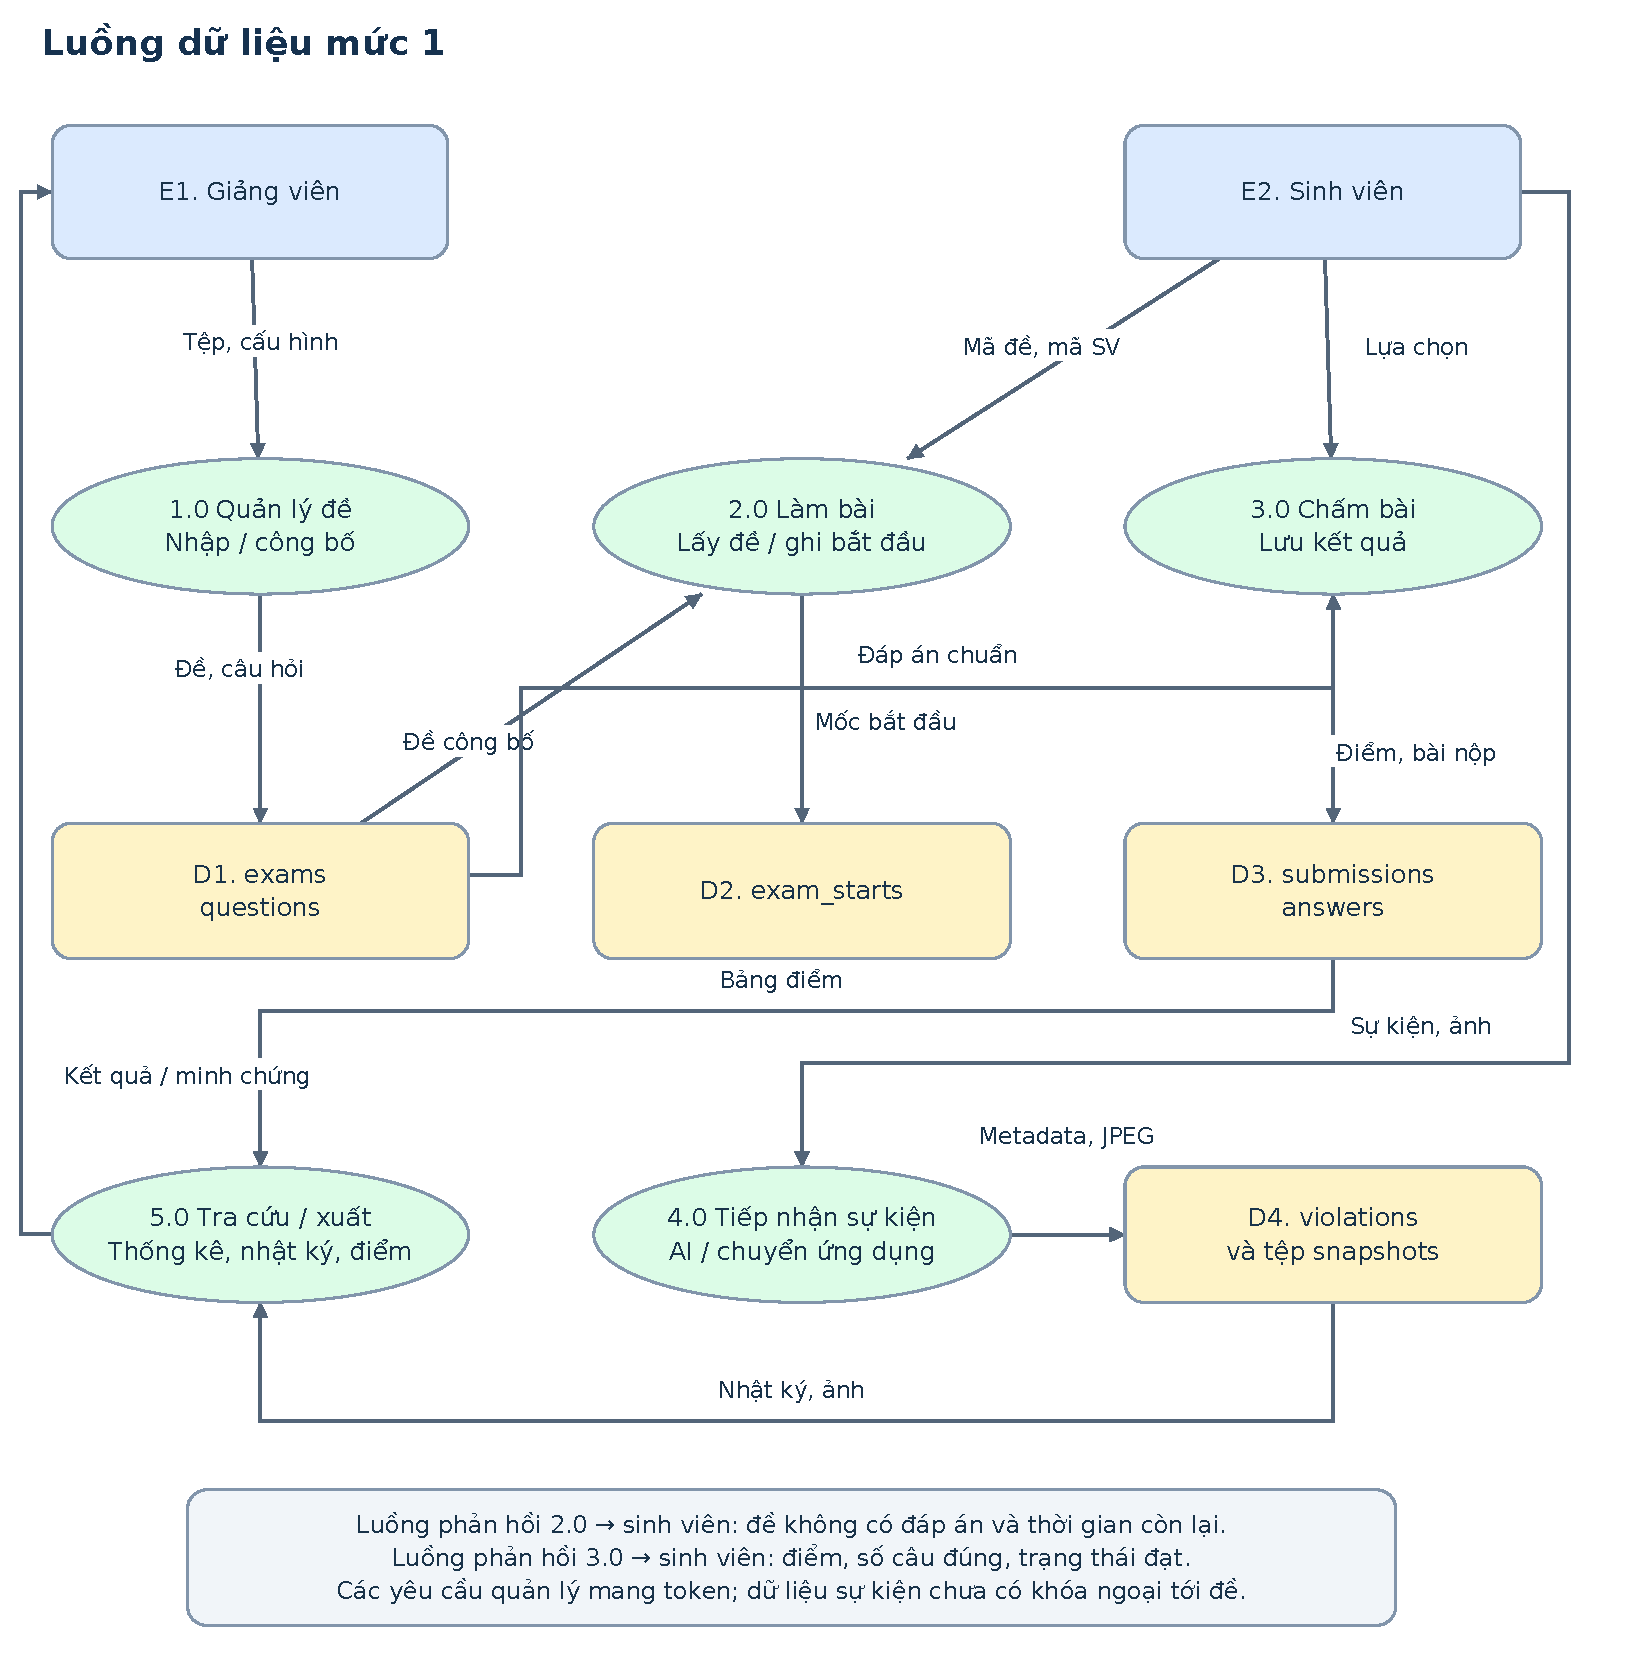
\includegraphics[width=\textwidth,height=0.70\textheight,keepaspectratio]{diagrams/05-dfd.pdf}
\caption{Luồng dữ liệu mức 1 của EduShield AI.}\label{fig:05-dfd}
\end{figure}

\clearpage
\subsection{Mô hình dữ liệu quan hệ}
ERD bổ sung exam\_starts và các quan hệ khóa ngoại thực tế. Đường đứt tới violations là phép ghép logic theo mã sinh viên và thời gian, không phải quan hệ được CSDL cưỡng chế.
\begin{figure}[H]
\centering
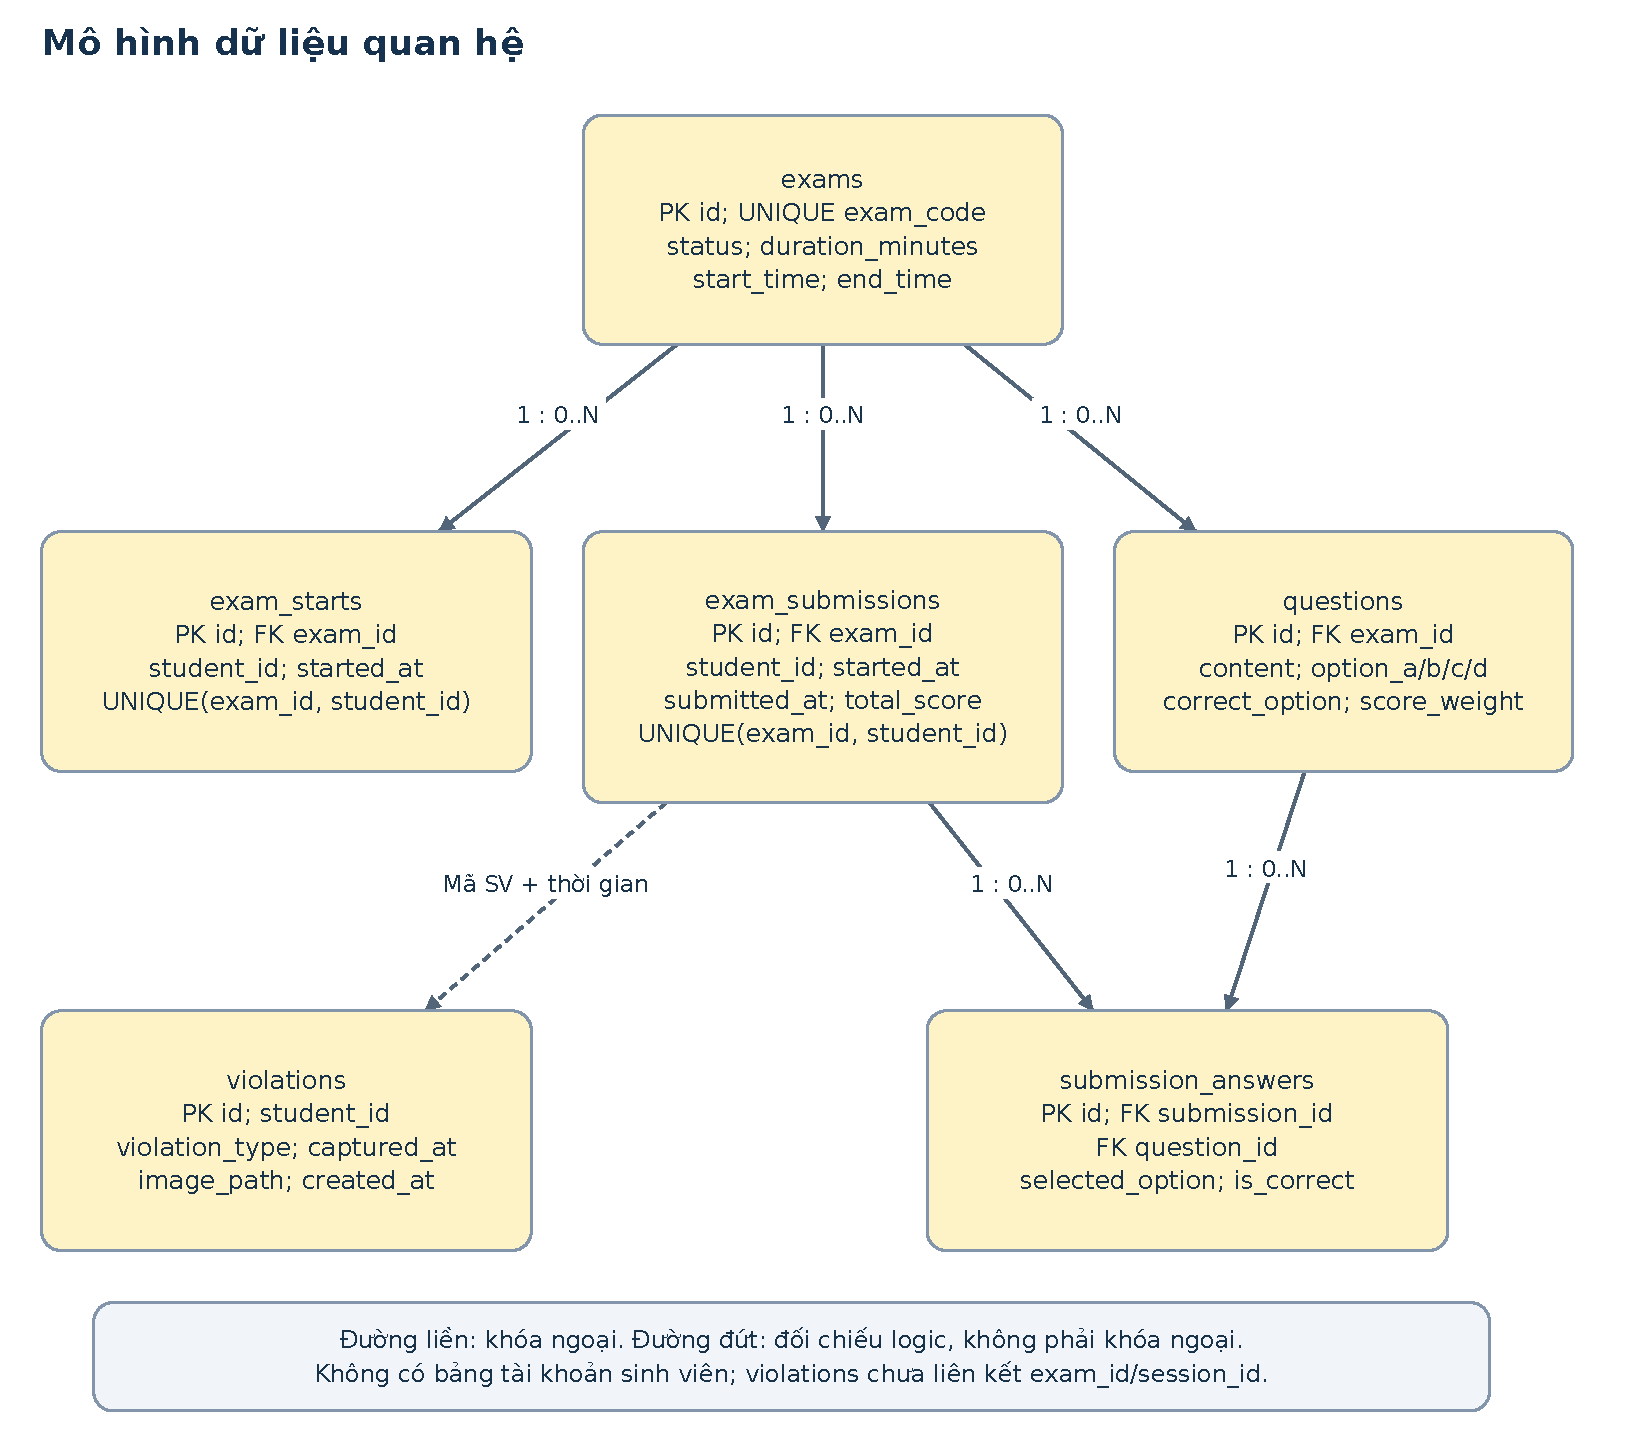
\includegraphics[width=\textwidth,height=0.70\textheight,keepaspectratio]{diagrams/06-erd.pdf}
\caption{Mô hình dữ liệu quan hệ của EduShield AI.}\label{fig:06-erd}
\end{figure}

\clearpage
\subsection{Luồng hoạt động toàn hệ thống}
Luồng tổng thể nối việc chuẩn bị đề và tunnel với quá trình làm bài, giám sát song song, nộp và tra cứu kết quả. Các nhánh lỗi mạng/camera được giải thích ở phần triển khai và kiểm thử.
\begin{figure}[H]
\centering
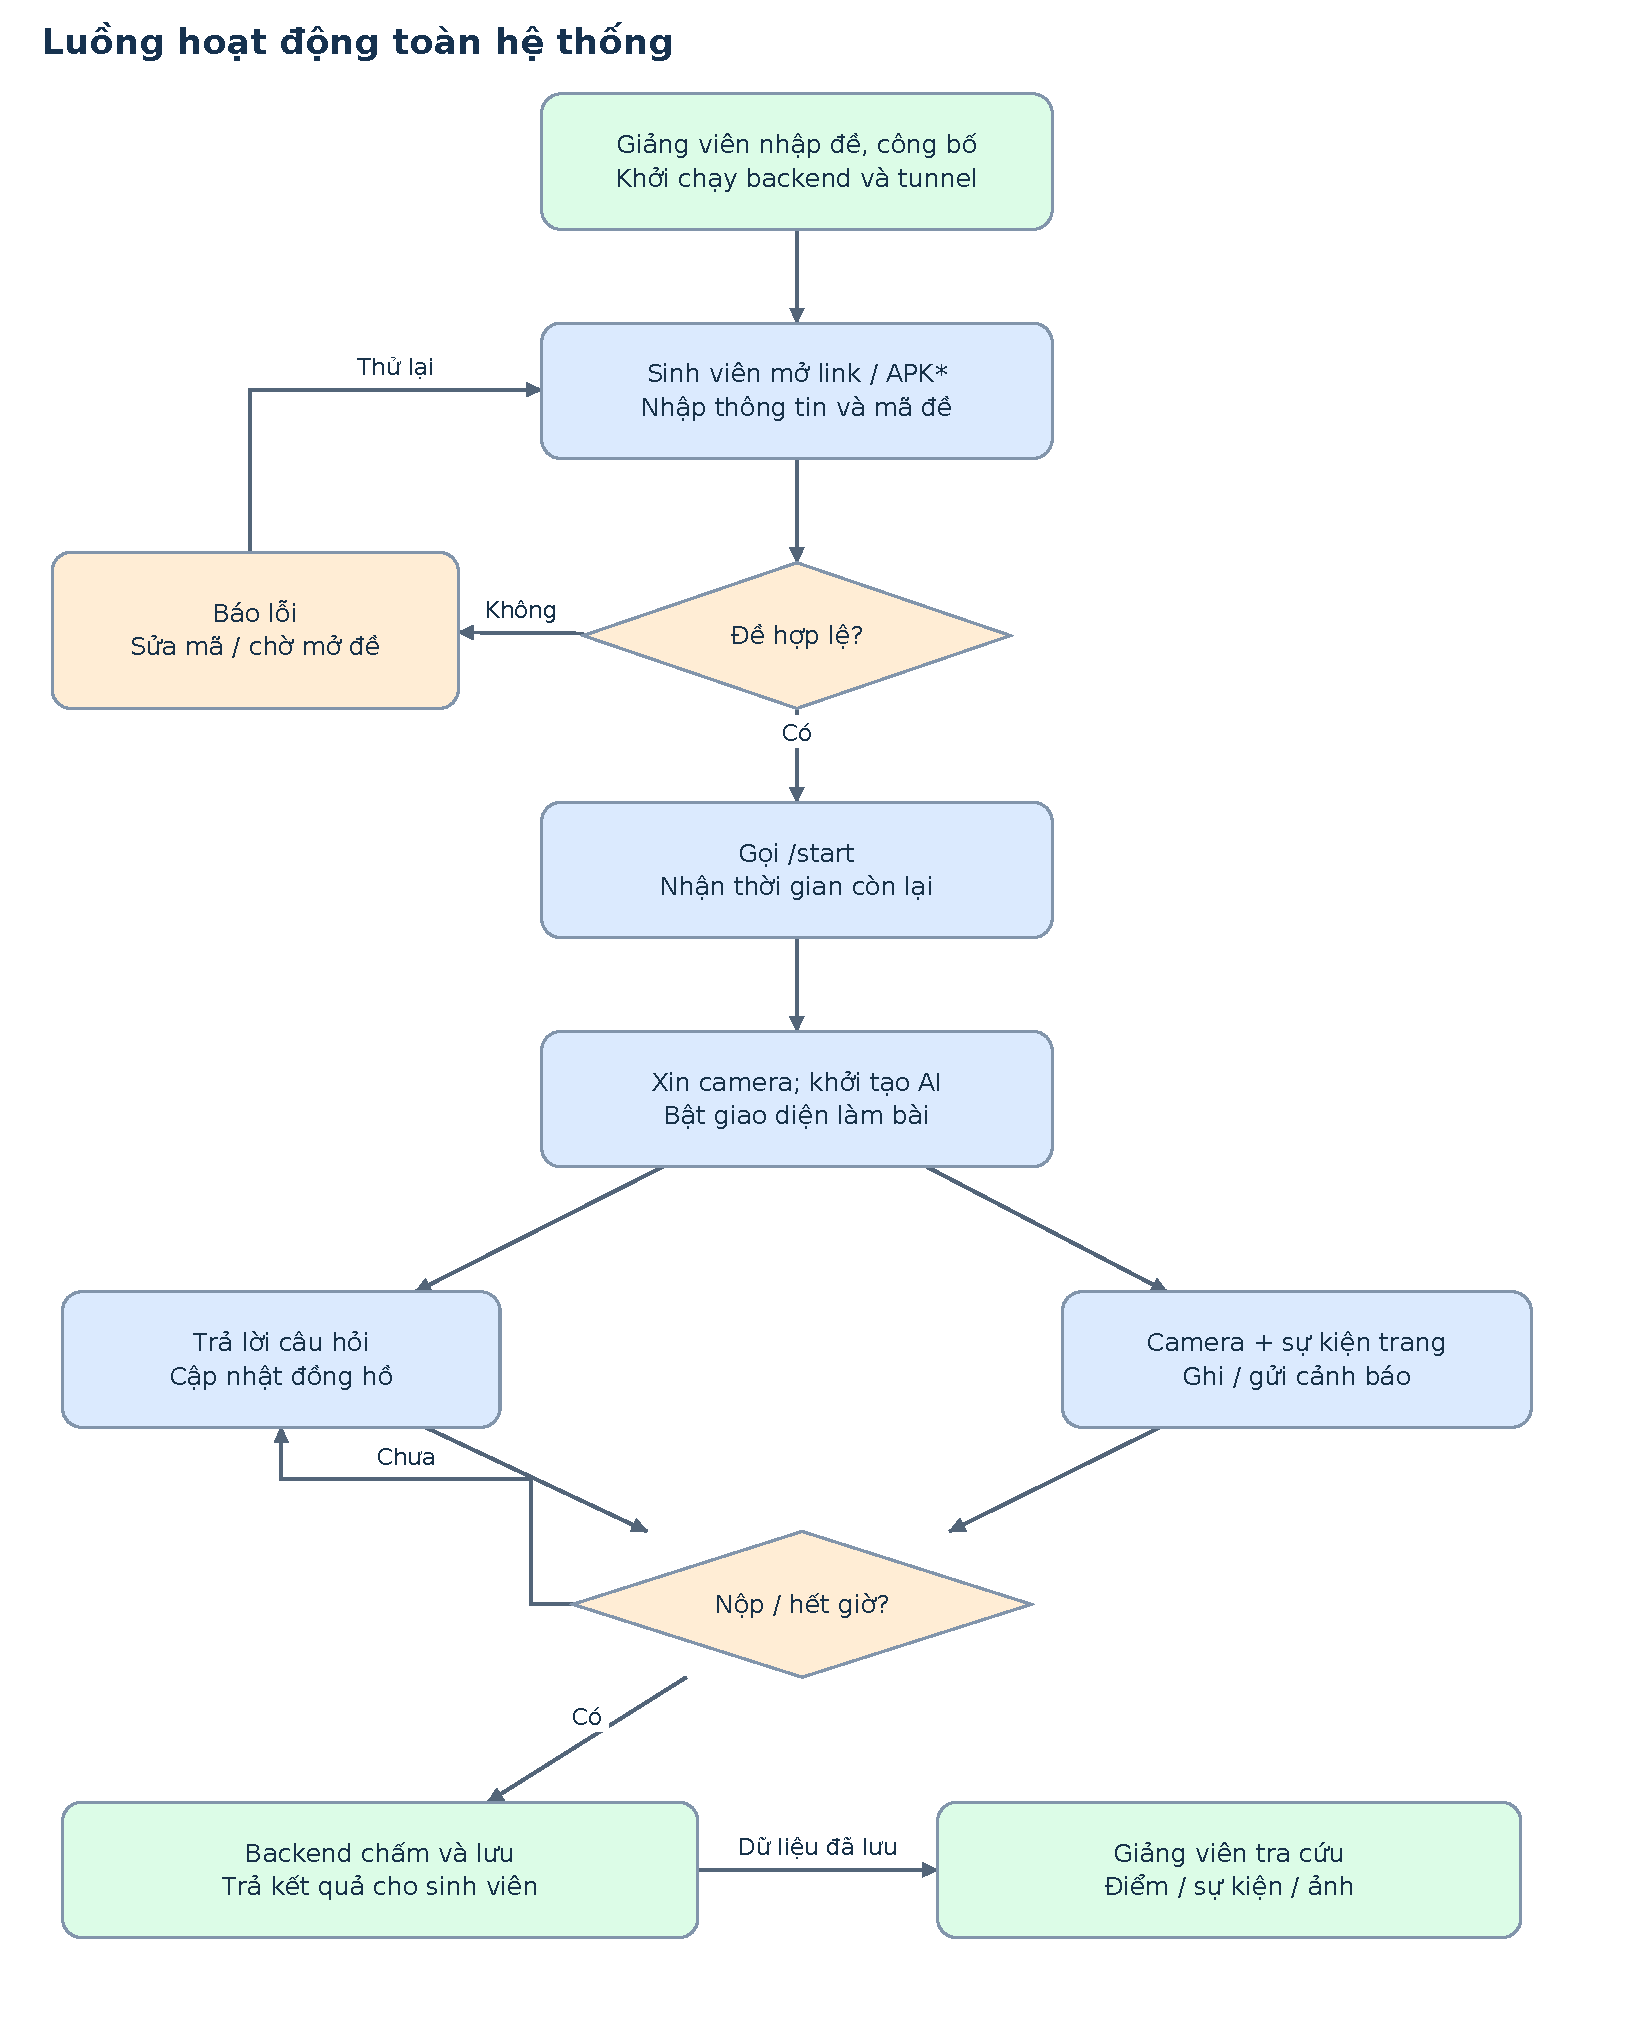
\includegraphics[width=\textwidth,height=0.70\textheight,keepaspectratio]{diagrams/07-activity.pdf}
\caption{Luồng hoạt động toàn hệ thống của EduShield AI.}\label{fig:07-activity}
\end{figure}

\clearpage
\subsection{Tuần tự bắt đầu và tiếp tục thời gian}
Thời gian còn lại do API start tính từ lần bắt đầu đầu tiên. Việc vào lại không phục hồi lựa chọn cũ; nhánh fallback vẫn cấp đủ thời lượng nếu API lỗi ngoài các trạng thái chặn đã nêu.
\begin{figure}[H]
\centering
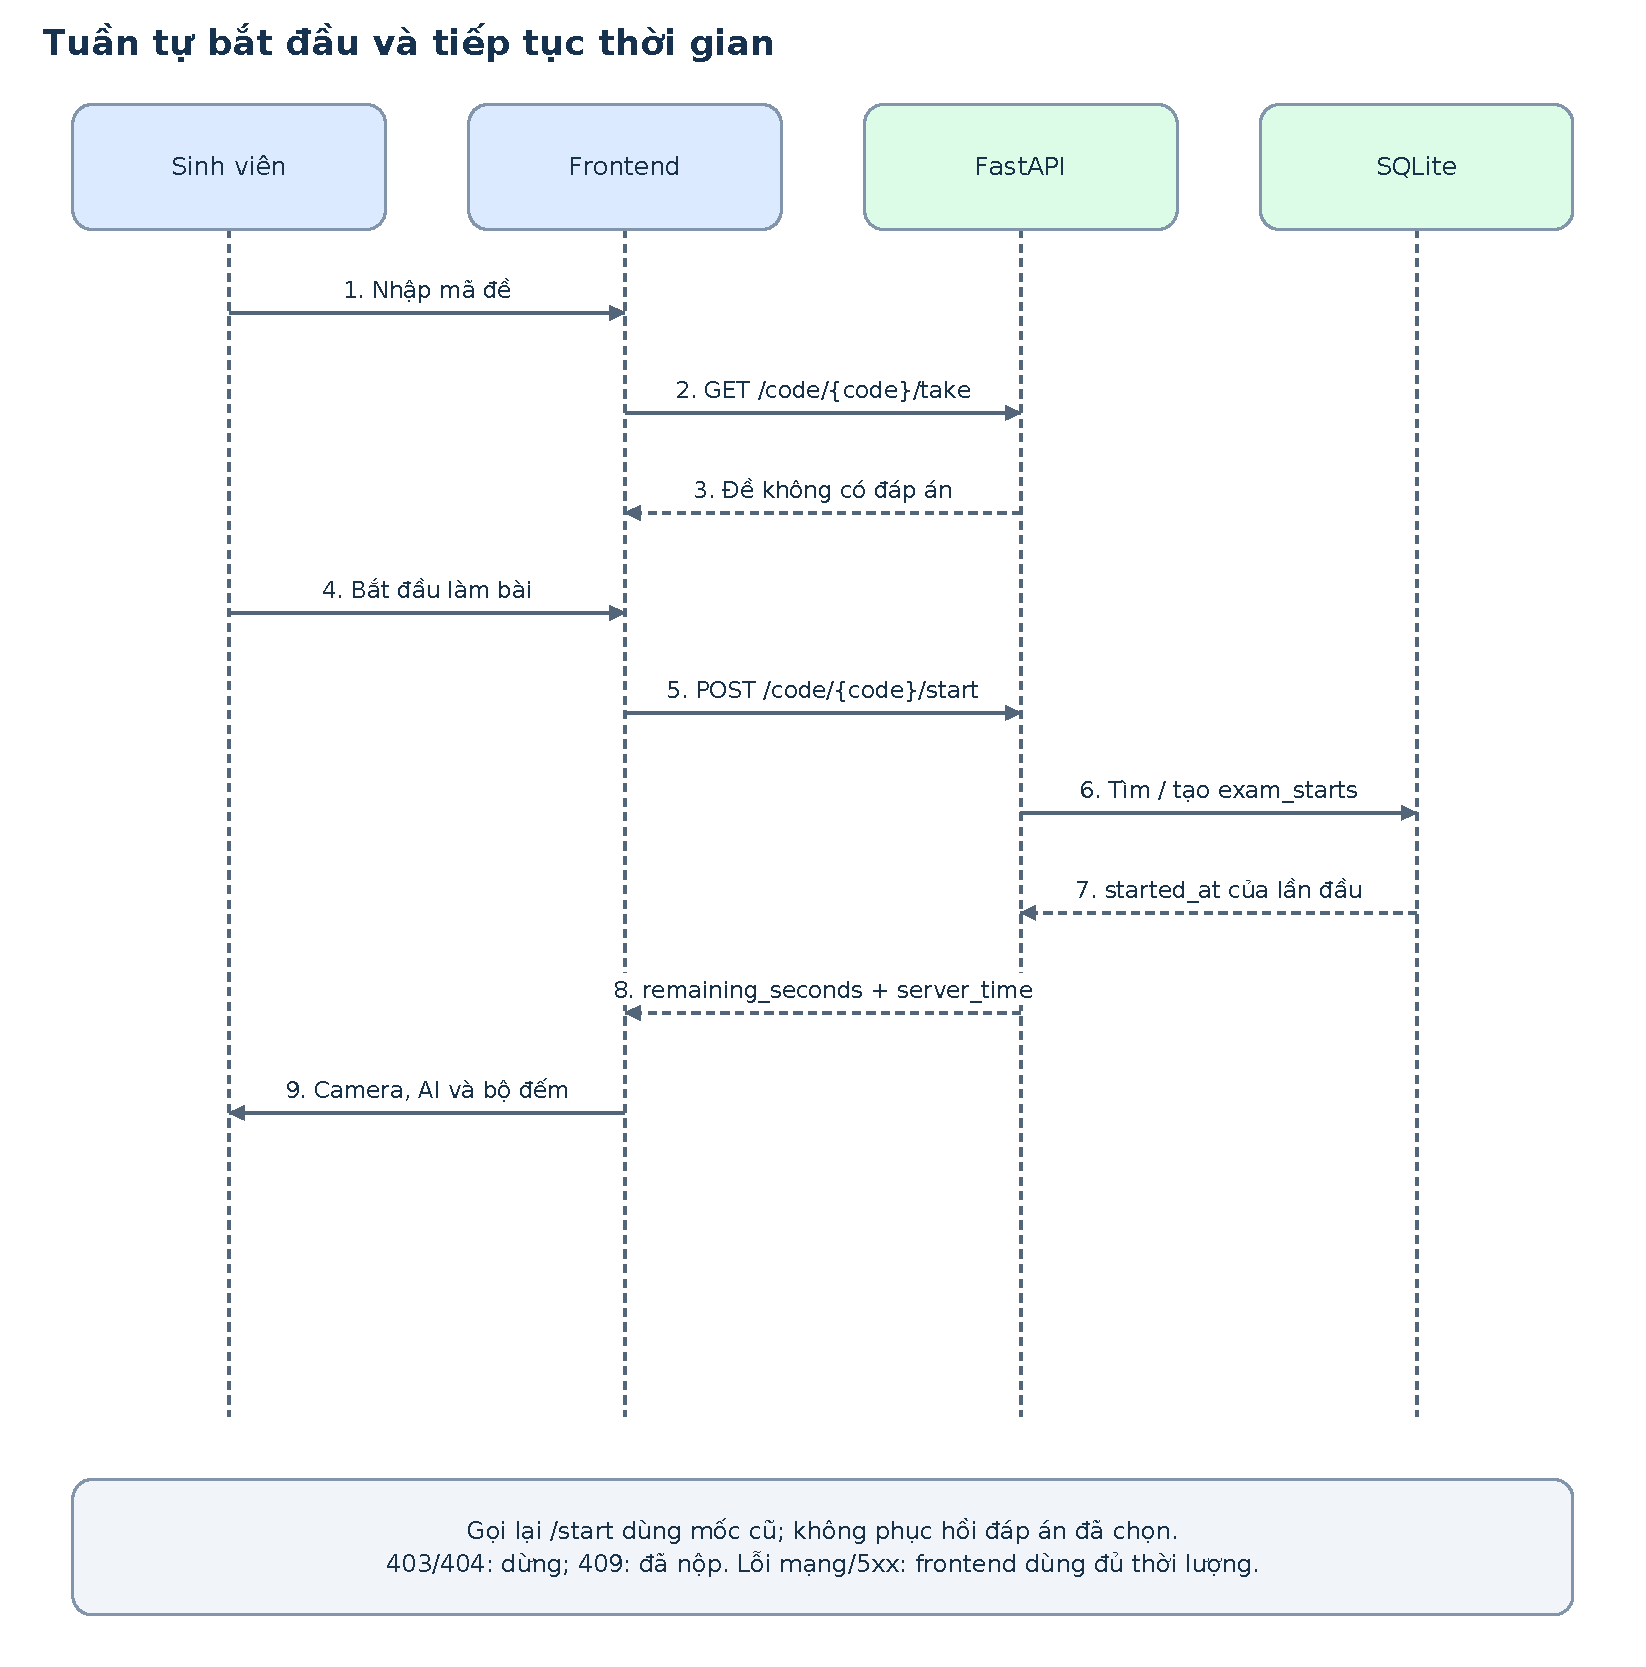
\includegraphics[width=\textwidth,height=0.70\textheight,keepaspectratio]{diagrams/08-seq-start.pdf}
\caption{Tuần tự bắt đầu và tiếp tục thời gian của EduShield AI.}\label{fig:08-seq-start}
\end{figure}

\clearpage
\subsection{Tuần tự ghi sự kiện và xem minh chứng}
Giảng viên đọc sự kiện bằng polling, không dùng WebSocket. Khi chuyển ứng dụng, camera có thể không cung cấp được ảnh; payload vẫn cho phép metadata không kèm ảnh.
\begin{figure}[H]
\centering
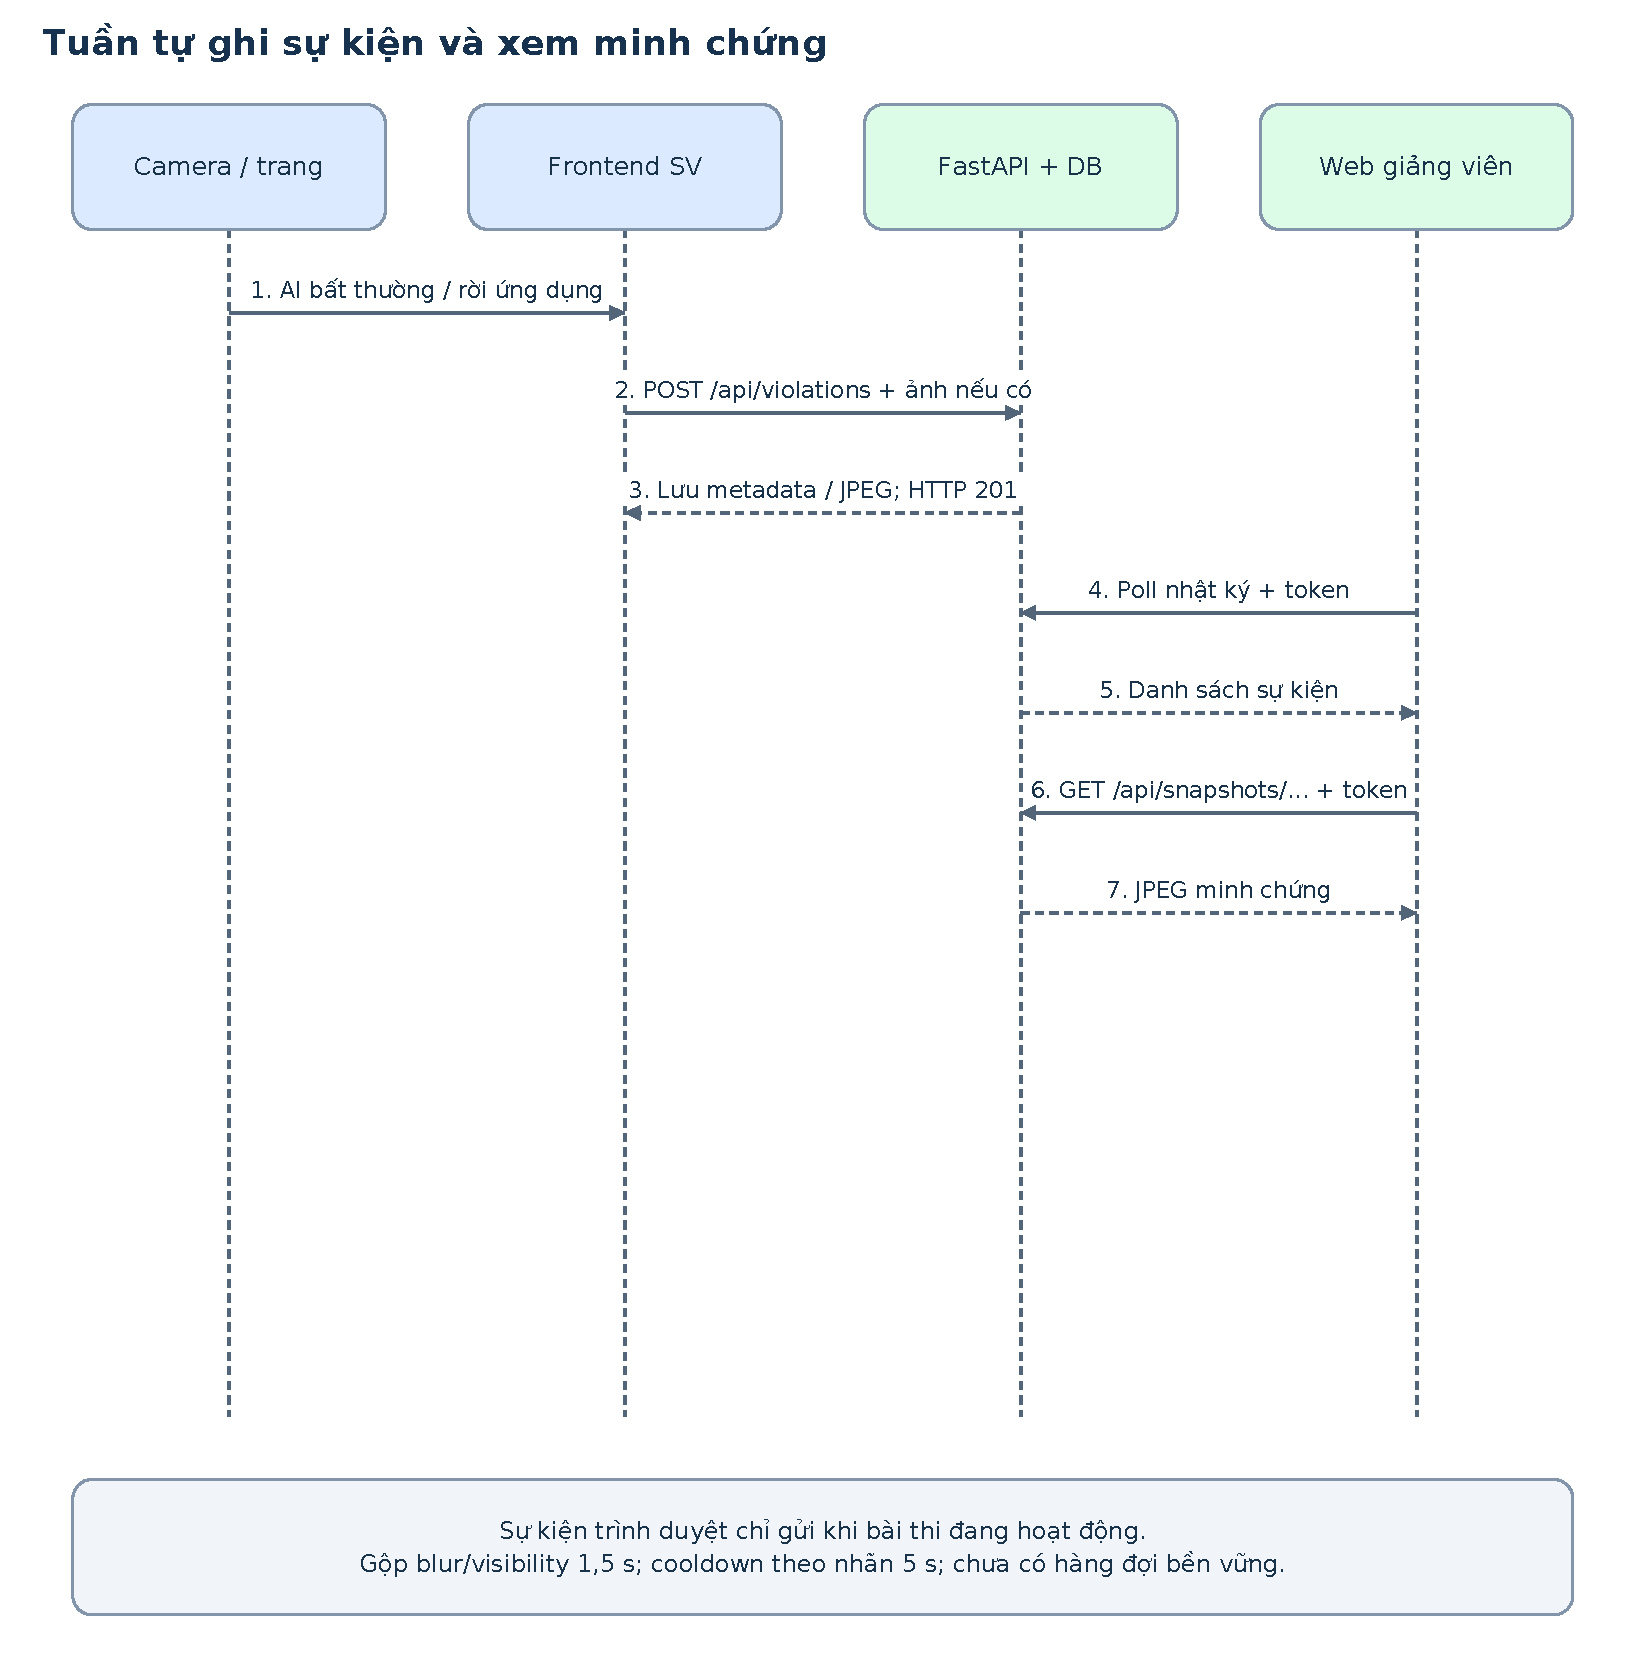
\includegraphics[width=\textwidth,height=0.70\textheight,keepaspectratio]{diagrams/09-seq-event.pdf}
\caption{Tuần tự ghi sự kiện và xem minh chứng của EduShield AI.}\label{fig:09-seq-event}
\end{figure}

\clearpage
\subsection{Tuần tự nộp và chấm bài}
Điểm được tính từ đáp án trong CSDL và ghi cùng chi tiết bài nộp. UNIQUE chống trùng là lớp bảo vệ cuối cùng; deadline chưa được cưỡng chế tại submit.
\begin{figure}[H]
\centering
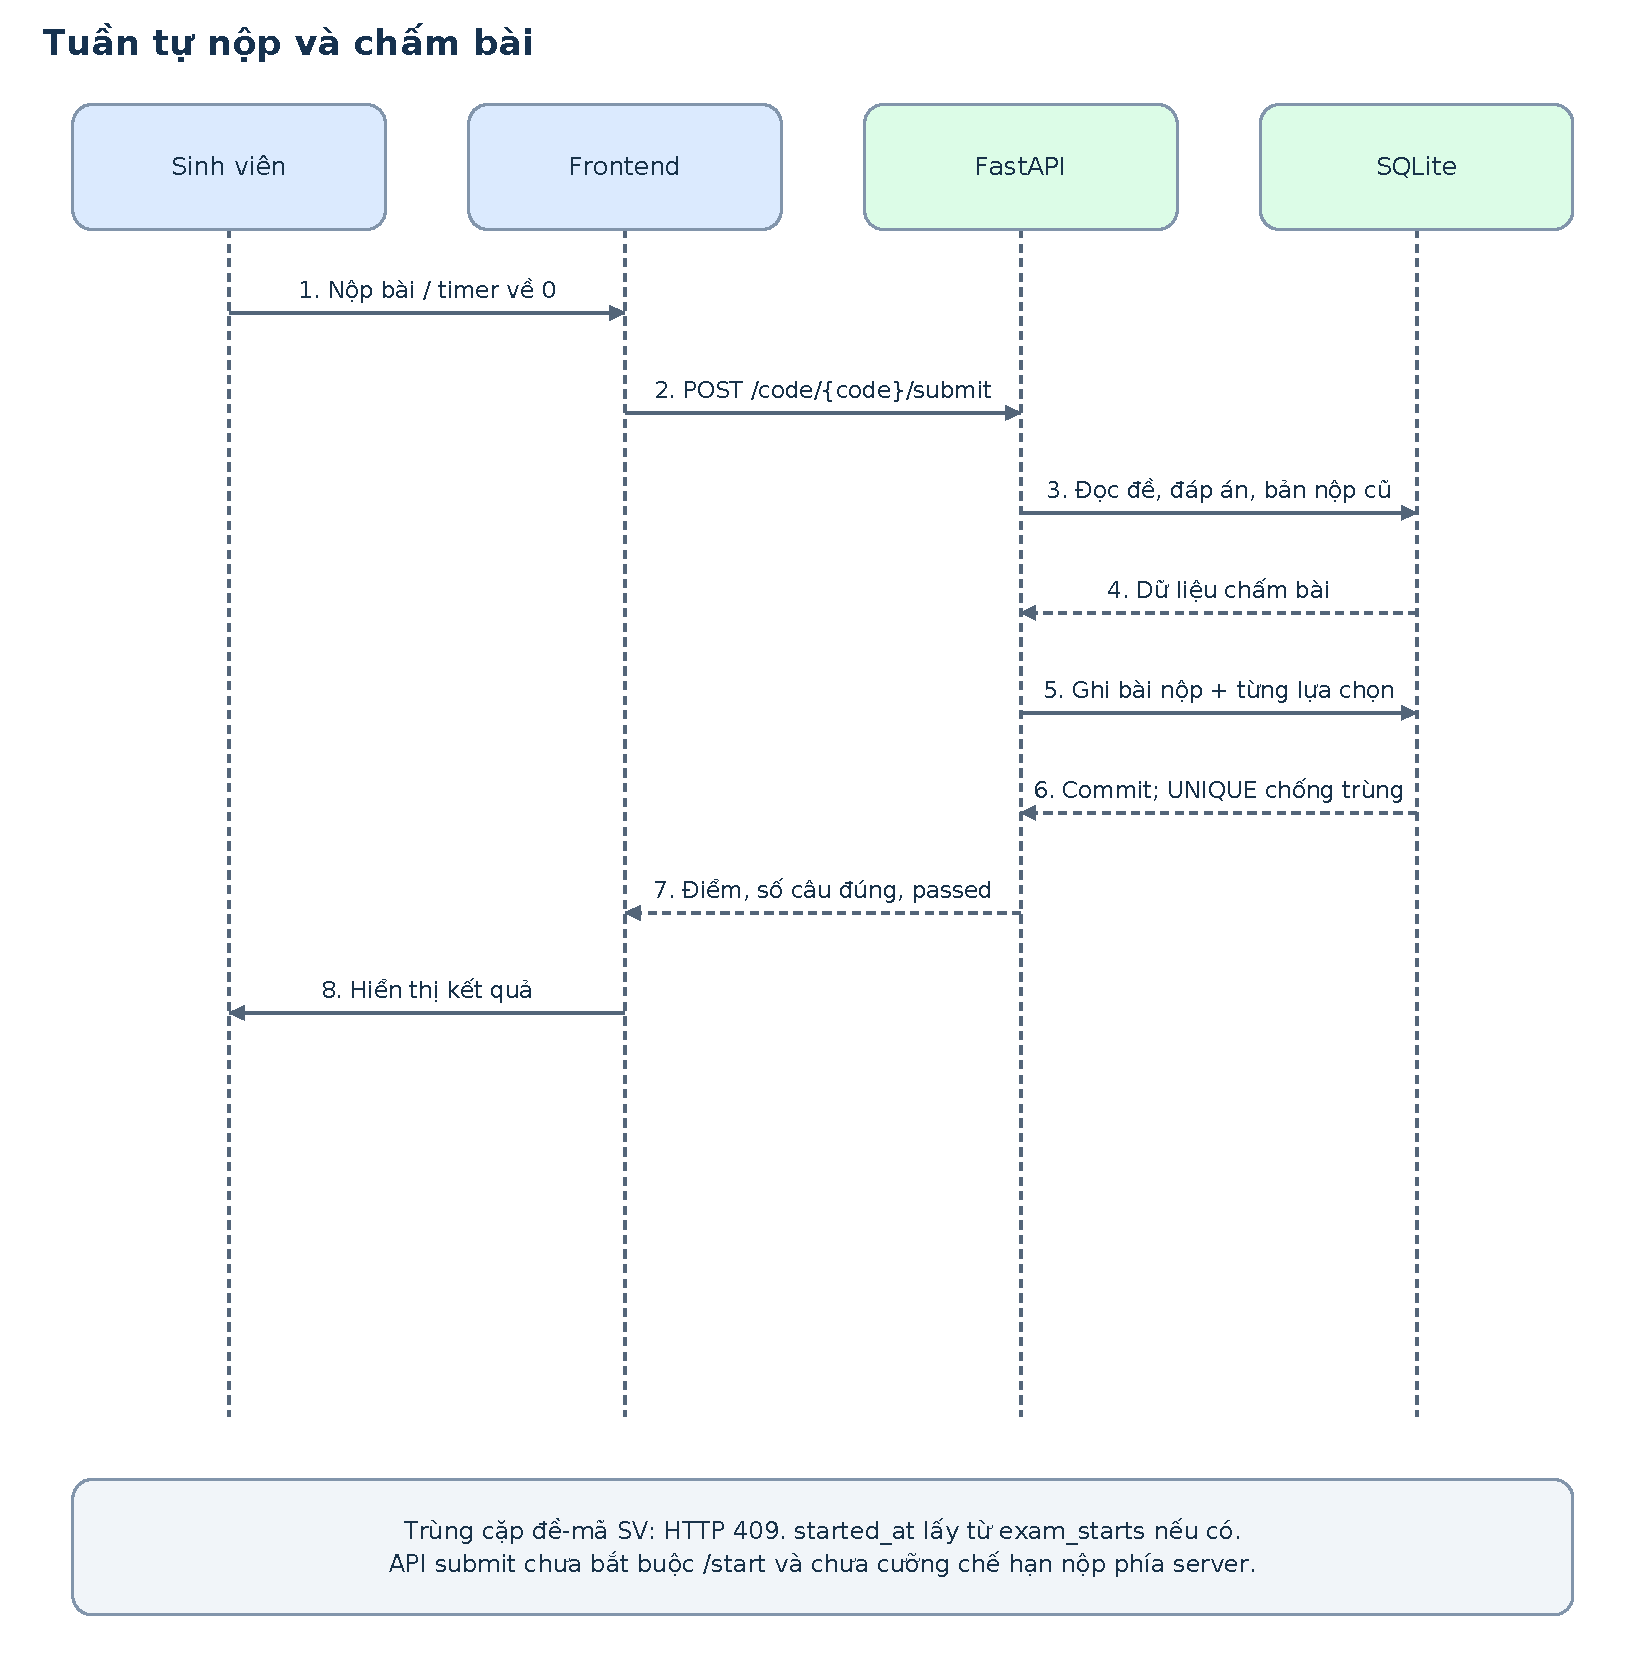
\includegraphics[width=\textwidth,height=0.70\textheight,keepaspectratio]{diagrams/10-seq-submit.pdf}
\caption{Tuần tự nộp và chấm bài của EduShield AI.}\label{fig:10-seq-submit}
\end{figure}

\clearpage
\subsection{Trạng thái tương tác của bài thi}
Đây là trạng thái tương tác của giao diện, không phải tập trạng thái lưu nguyên dạng trong CSDL. Xuống nền không có nghĩa là backend tạm dừng thời gian thi.
\begin{figure}[H]
\centering
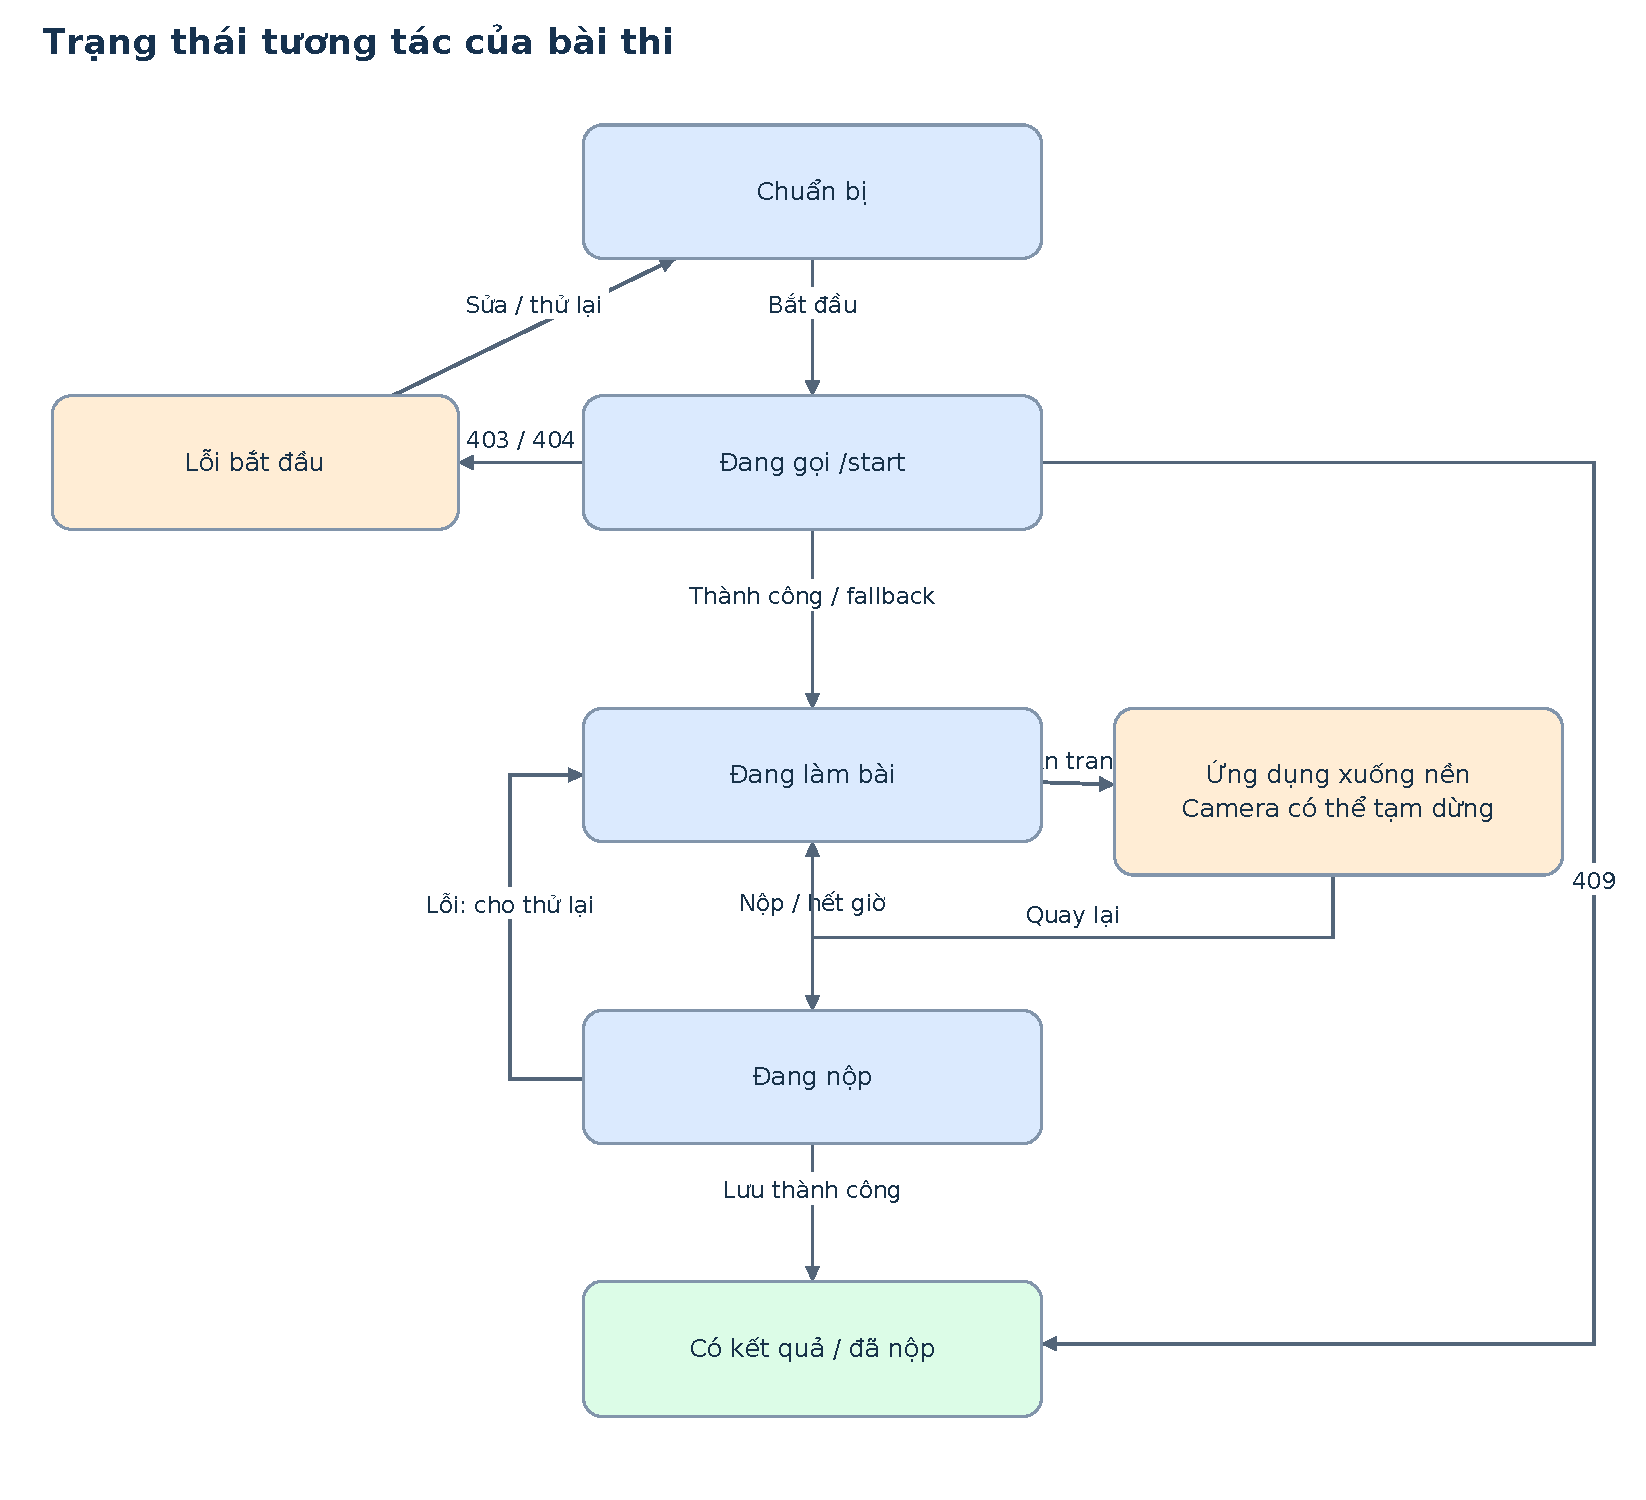
\includegraphics[width=\textwidth,height=0.70\textheight,keepaspectratio]{diagrams/11-state.pdf}
\caption{Trạng thái tương tác của bài thi của EduShield AI.}\label{fig:11-state}
\end{figure}

\clearpage
\subsection{Luồng giám sát AI tại máy khách}
Luồng AI giữ thứ tự ưu tiên nhãn và cooldown. Chu kỳ mobile giảm số lượt suy luận; không suy ra độ chính xác hoặc độ trễ thực đo chỉ từ thông số này.
\begin{figure}[H]
\centering
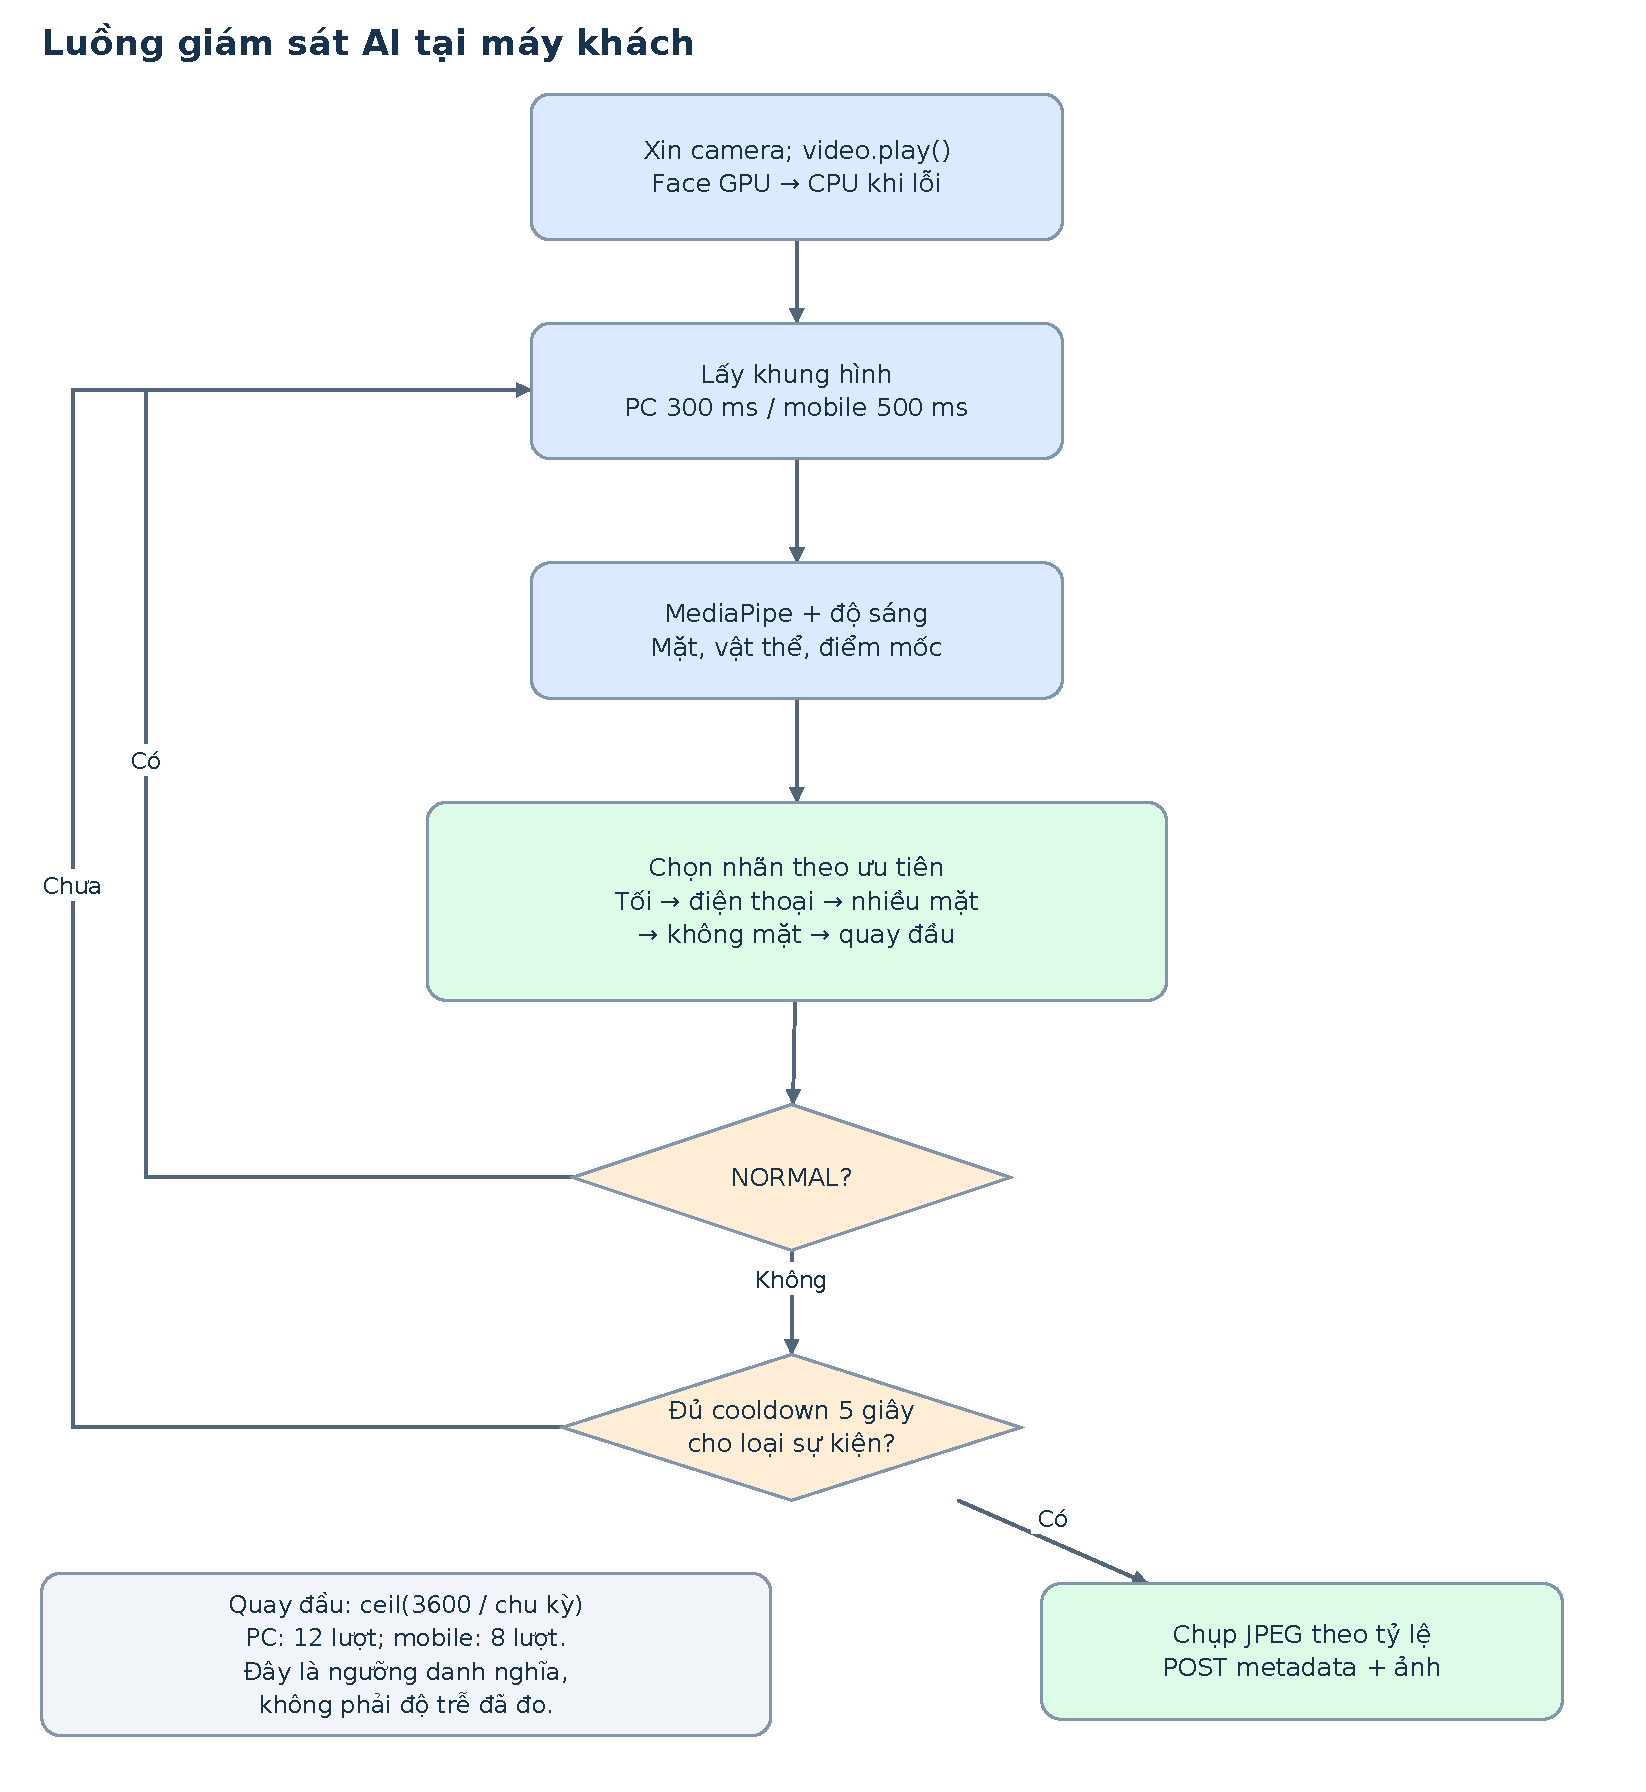
\includegraphics[width=\textwidth,height=0.70\textheight,keepaspectratio]{diagrams/12-ai-flow.pdf}
\caption{Luồng giám sát AI tại máy khách của EduShield AI.}\label{fig:12-ai-flow}
\end{figure}
